\documentclass[12pt,a4paper]{article}
%
%	STARWARE - Stile base per la scrittura di documenti interni in LaTex
%

%
%	Pacchetti globali
%	Fare qui eventuali aggiunte!
%
\usepackage[utf8]{inputenc}
\usepackage[italian]{babel}
\usepackage[babel]{csquotes}
\usepackage{url}
\usepackage{graphicx}
\usepackage[colorlinks]{hyperref}
\usepackage{lastpage}
\usepackage{fancyhdr}
\usepackage[top=1cm,bottom=4cm,left=80pt,right=80pt]{geometry} %disegna la linea
\usepackage{listings} %per grandi porzioni di codice
\usepackage{color}
\usepackage[table]{xcolor}
\usepackage{booktabs,tabularx}
\usepackage{makeidx}
\usepackage{fixltx2e}
\usepackage{hyperref}
\usepackage{enumitem}
\usepackage{color}
\usepackage[T1]{fontenc}
\usepackage{float}
\usepackage{svg}
\usepackage{amsmath}
\usepackage[toc]{glossaries}
\usepackage{dirtree}
\usepackage{listings}

\makeglossaries

\bibliographystyle{alpha}

%
%	VARIABILI GLOBALI
%
\newcommand{\nomeGruppo}{StarWare}
\newcommand{\mailGruppo}{starware.swe@gmail.com}
\newcommand{\uni}{Universit\`{a} degli Studi di Padova}
\newcommand{\uniAA}{2015/2016}
\newcommand{\Cardin}{Prof. Riccardo Cardin}
\newcommand{\Vardanega}{Prof. Tullio Vardanega}
\newcommand{\Zucchetti}{Zucchetti S.p.a.}
\newcommand{\prj}{Quizzipedia}
\newcommand{\prjL}{Quizzipedia: software per la gestione di questionari}

\newcommand{\AVI}{Alessio Vitella}
\newcommand{\AVE}{Andrea Venier}
\newcommand{\NDC}{Nicola De Cao}
\newcommand{\IB}{Igor Baylyak}
\newcommand{\WS}{Walter Sandon}
\newcommand{\TP}{Thomas Pigarelli}
\newcommand{\AB}{Anna Bonaldo}

\newcommand{\mgls}[1]{\gls{#1}\textsubscript{G}}
\newcommand{\mglspl}[1]{\glspl{#1}\textsubscript{G}}
\newcommand{\mGls}[1]{\Gls{#1}\textsubscript{G}}
\newcommand{\mGlspl}[1]{\Glspl{#1}\textsubscript{G}}

\newcommand{\AM}{\emph{\mGls{amministratore}}}
\newcommand{\AN}{\emph{\mGls{analista}}}
\newcommand{\PG}{\emph{\mGls{progettista}}}
\newcommand{\PR}{\emph{\mGls{programmatore}}}
\newcommand{\VR}{\emph{\mGls{verificatore}}}
\newcommand{\PM}{\emph{\mGls{project manager}}}

\newcommand{\AMpl}{\emph{\mGlspl{amministratore}}}
\newcommand{\ANpl}{\emph{\mGlspl{analista}}}
\newcommand{\PGpl}{\emph{\mGlspl{progettista}}}
\newcommand{\PRpl}{\emph{\mGlspl{programmatore}}}
\newcommand{\VRpl}{\emph{\mGlspl{verificatore}}}
\newcommand{\PMpl}{\emph{\mGlspl{project manager}}}

\newcommand{\RR}{\emph{\mGls{revisione dei requisiti}}}
\newcommand{\RA}{\emph{\mGls{revisione di accettazione}}}
\newcommand{\RP}{\emph{\mGls{revisione di progettazione}}}
\newcommand{\RQ}{\emph{\mGls{revisione di qualifica}}}

\newcommand{\NdP}{\emph{\mGls{norme di progetto}}}
\newcommand{\SdF}{\emph{\mGls{stidio di fattibilita}}}
\newcommand{\AdR}{\emph{\mGls{analisi dei requisiti}}}
\newcommand{\PdP}{\emph{\mGls{piano di progetto}}}
\newcommand{\PdQ}{\emph{\mGls{piano di qualifica}}}

\newcommand{\latex}[1]{\texttt{#1}}
\newcommand{\fileName}[1]{\texttt{#1}}
\newcommand{\filePath}[1]{\texttt{#1}}
\newcommand{\TODO}[1]{\texttt{\large \color{red} \underline{TODO: #1}}}

\newcommand{\licenza}{GNU GENERAL PUBLIC LICENSE V2}

%per compilare il template usare questi sotto e commentare glia altri:
%\newcommand{\logoLungo}{../imgs/logoLungo.png}
%\newcommand{\logoGrande}{../imgs/logoGrande.png}
\newcommand{\logoLungo}{../../../template/imgs/logoLungo.png}
\newcommand{\logoGrande}{../../../template/imgs/logoGrande.png}

%
%	Setup stili
%

\newcommand{\HRule}{\rule{\linewidth}{0.5mm}}

\definecolor{dkgreen}{rgb}{0,0.6,0}
\definecolor{gray}{rgb}{0.5,0.5,0.5}
\definecolor{mauve}{rgb}{0.58,0,0.82}
\definecolor{light}{RGB}{255,255,190}

%
%	Setup di pagina
%

%colorazione link
\hypersetup
{
	colorlinks=true,
	linkcolor=black,
	urlcolor=blue,
	citecolor=blue
}

%	Setup Header + Footer

\pagestyle{fancy}
\setlength{\headheight}{2cm} %settato grandezza header

\renewcommand{\footrulewidth}{0.5pt} %ridefinisco il valore della riga di intestazione
\renewcommand{\headrulewidth}{0.5pt} %ridefinisco il valore della riga di pie' di pagina
\addtolength{\headwidth}{\marginparsep}
\addtolength{\headwidth}{\marginparwidth}

\fancyhead{} %annulla head di default
\fancyfoot{} %annulla foot di default

%	Logo intestazione
\lhead{
\includegraphics[scale=0.12]{\logoLungo}}


%	footer
\cfoot{
	\uni \ - \uniAA \\
	\href{mailto:\mailGruppo}{\mailGruppo}\\
	{\tiny Questo documento è distribuito sotto licenza {\licenza}}
}
\rfoot{
	\thepage\ di \pageref{LastPage}
}


% test subsubsubsection

\usepackage{titlesec}
\usepackage{hyperref}

\titleclass{\subsubsubsection}{straight}[\subsection]

\newcounter{subsubsubsection}[subsubsection]
\renewcommand\thesubsubsubsection{\thesubsubsection.\arabic{subsubsubsection}}
\renewcommand\theparagraph{\thesubsubsubsection.\arabic{paragraph}} % optional; useful if paragraphs are to be numbered

\titleformat{\subsubsubsection}
  {\normalfont\normalsize\bfseries}{\thesubsubsubsection}{1em}{}
\titlespacing*{\subsubsubsection}
{0pt}{3.25ex plus 1ex minus .2ex}{1.5ex plus .2ex}

\makeatletter
\renewcommand\paragraph{\@startsection{paragraph}{5}{\z@}%
  {3.25ex \@plus1ex \@minus.2ex}%
  {-1em}%
  {\normalfont\normalsize\bfseries}}
\renewcommand\subparagraph{\@startsection{subparagraph}{6}{\parindent}%
  {3.25ex \@plus1ex \@minus .2ex}%
  {-1em}%
  {\normalfont\normalsize\bfseries}}
\def\toclevel@subsubsubsection{4}
\def\toclevel@paragraph{5}
\def\toclevel@paragraph{6}
\def\l@subsubsubsection{\@dottedtocline{4}{7em}{4em}}
\def\l@paragraph{\@dottedtocline{5}{10em}{5em}}
\def\l@subparagraph{\@dottedtocline{6}{14em}{6em}}
\makeatother

\setcounter{secnumdepth}{4}
\setcounter{tocdepth}{4}


%pdflatex -synctex=1 -interaction=nonstopmode %.tex|makeglossaries %|pdflatex -synctex=1 -interaction=nonstopmode %.tex|pdflatex -synctex=1 -interaction=nonstopmode %.tex
\makeglossary

\newglossaryentry{responsabile} {
	name=responsabile,
	description={è il responsabile della gestione, pianificazione e realizzazione del progetto},
	plural=Responsabili
}

\newglossaryentry{verificatore} {
	name=verificatore,
	description={è il responsabile dell'attività di verifica},
	plural=Verificatori
}

\newglossaryentry{programmatore} {
	name=programmatore,
	description={è responsabile delle attività di codifica miranti alla realizzazione del prodotto e delle componenti di ausilio necessarie per l'esecuzione delle prove di verifica e validazione},
	plural=programmatori
}

\newglossaryentry{progettista} {
	name=progettista,
	description={è responsabile delle attività di progettazione},
	plural=Progettisti
}

\newglossaryentry{analista} {
	name=analista,
	description={è responsabile delle attività di analisi. },
	plural=Analisti
}

\newglossaryentry{amministratore} {
	name=amministratore,
	description={è responsabile dell'efficienza e dell'operatività dell'ambiente di sviluppo; si occupa della redazione e attuazione di piani e procedure di gestione della qualità; inoltre gestisce l'archivio della documentazione del progetto},
	plural=Amministratori
}

\newglossaryentry{revisione dei requisiti} {
	name=revisione dei requisiti,
	description={è una revisione formale che determina l'accesso del gruppo al progetto didattico e la concordanza con il cliente di una visione condivisa del prodotto atteso}
}

\newglossaryentry{revisione di accettazione} {
	name=revisione di accettazione,
	description={è una revisione formale per l'accertamento del soddisfacimento di tutti i requisiti e il completamento del progetto}
}

\newglossaryentry{revisione di progettazione} {
	name=revisione di progettazione,
	description={è una revisione di progresso che accerta la realizzabilità del prodotto e informa il cliente sulle caratteristiche del prodotto}
}

\newglossaryentry{revisione di qualifica} {
	name=revisione di qualifica,
	description={è una revisione di progresso che approva l'esito finale delle verifiche e attiva la fase di validazione}
}

\newglossaryentry{analisi} {
	name=analisi,
	description={è il periodo di preparazione e produzioni di documenti che precede la Revisione dei requisiti}
}

\newglossaryentry{progettazione} {
	name=progettazione,
	description={è il periodo che intercorre tra la Revisione dei requisiti e la Revisione di progettazione}
}

\newglossaryentry{codifica} {
	name=codifica,
	description={è il periodo che intercorre tra la Revisione di progettazione e la Revisione di qualifica}
}

\newglossaryentry{validazione} {
	name=validazione,
	description={è il periodo che intercorre tra la Revisione di qualifica e la Revisione di accettazione}
}

\newglossaryentry{repository} {
	name=repository,
	description={è dove i file sono memorizzati, spesso su un server}
}

\newglossaryentry{ruolo} {
	name=ruolo,
	description={una delle figure professionali che una persona fisica interpreta nel corso del progetto. I ruoli sono: responsabile, amministratore, analista, progettista, programmatore e verificatore},
    plural=ruoli
}

\newglossaryentry{svg} {
	name=SVG,
	description={è un formato per la visualizzazione di oggetti in grafica vettoriale. Per maggiori informazioni si veda \href{https://it.wikipedia.org/wiki/Scalable_Vector_Graphics}{qui}}
}

\newglossaryentry{png} {
	name=PNG,
	description={abbreviazione di Portable Network Graphics, è un formato di file per memorizzare immagini. Per ulteriori informazioni si veda \href{http://it.wikipedia.org/wiki/Portable_Network_Graphics}{qui}}
}

\newglossaryentry{pdf} {
	name=PDF,
	description={è un formato di file basato su un linguaggio di descrizione di pagina sviluppato da Adobe Systems nel 1993 per rappresentare documenti in modo indipendente dall’hardware e dal software utilizzati per generarli o per visualizzarli. Per ulteriori informazioni si veda \href{http://it.wikipedia.org/wiki/Portable_Document_Format}{qui}}
}

\newglossaryentry{uml} {
	name=UML,
	description={è un linguaggio di modellazione e specifica basato sul paradigma object-oriented. Per ulteriori informazioni si veda \href{http://it.wikipedia.org/wiki/Unified_Modeling_Language}{qui}}
}

\newglossaryentry{walkthrough} {
	name=walkthrough,
    description={consiste nella lettura di un documento o codice cercando errori ed anomalie senza un'idea precisa di quali tipi di errori sarà possibile trovare}
}

\newglossaryentry{lista di controllo} {
	name=lista di controllo,
	description={è un elenco di cose da fare per eseguire una determinata attività}
}

\newglossaryentry{inspection} {
	name=inspection,
	description={è la lettura mirata di un documento o codice cercando errori specifici}
}

\newglossaryentry{milestone} {
	name=milestone,
	description={momento saliente nello sviluppo di un prodotto software per la quale devono essere pronti documenti e/o funzionalità}
}

\newglossaryentry{ticket} {
	name=ticket,
	description={rappresenta un compito nell'organizzazione e distribuzione del lavoro all'interno del progetto},
	plural=tickets
}

\newglossaryentry{commit} {
	name=commit,
	description={è la copia di modifiche fatte su file locali verso la repository remota. Esso rappresenta anche un particolare stato della repository nel tempo}
}

\newglossaryentry{versionamento} {
	name=versionamento,
	description={è la gestione di un versioni multiple di un insieme di informazioni. Per maggiori informazioni si veda \href{http://it. wikipedia.org/wiki/Controllo_versione}{qui}}
}

\newglossaryentry{task} {
	name=task,
	description={è un compito secondo la definizione dello standard IEEE 12207},
	plural=tasks
}

\newglossaryentry{attivita} {
	name=attivita,
	description={è un insieme di task}
}

\newglossaryentry{redattore} {
	name=redattore,
	description={colui che redige un documento},
	plural=redattori
}

\newglossaryentry{proponente} {
	name=proponente,
	description={colui che ha proposto al committente un capitolato d'appalto}
}

\newglossaryentry{committente} {
	name=committente,
	description={colui che assegna un compito. In questo caso è il Professor Tullio Vardanega}
}

\newglossaryentry{quality assurance} {
	name=quality assurance,
	description={è l'insieme delle attività volte a garantire il soddisfacimento degli obiettivi della qualità}
}

\newglossaryentry{telegram} {
	name=telegram,
	description={è un servizio di messaggistica istantanea utilizzato dal gruppo per comunicazioni interne. Per maggiori informazioni si veda \href{https://it.wikipedia.org/wiki/Telegram_(software)}{qui}}
}

\newglossaryentry{browser} {
	name=browser,
	description={è un'applicazione per il recupero, la presentazione e la navigazione di risorse web}
}

\newglossaryentry{google drive} {
	name=Google Drive,
	description={è un servizio di memorizzazione e sincronizzazione online introdotto da Google il 24 aprile 2012. Per maggiori informazioni si veda \href{https://it.wikipedia.org/wiki/Google_Drive}{qui}}
}

\newglossaryentry{skype} {
	name=Skype,
	description={è un software proprietario freeware di messaggistica istantanea e VoIP. Per maggiori informazioni si veda \href{https://it.wikipedia.org/wiki/Skype}{qui}}
}

\newglossaryentry{gantt} {
	name=Gantt,
	description={è un diagramma di supporto alla gestione dei progetti}
}

\newglossaryentry{projectlibre} {
	name=ProjectLibre,
	description={è un software di gestione progettuale}
}

\newglossaryentry{pert} {
	name=PERT,
	description={è uno strumento volto alla programmazione delle attività che compongono il progetto e, più in generale, alla gestione degli aspetti temporali di quest'ultimo}
}

\newglossaryentry{subtask} {
	name=subtask,
	description={è un task compreso all'interno di un altro task. La totalità di tutti i subtasks costituisce un intero task}
	plural=subtasks
}

\newglossaryentry{ticketing} {
	name=ticketing,
	description={procedura con la quale il Responsabile assegna un task}
}

\newglossaryentry{git} {
	name=git,
	description={è un sistema software di controllo di versione distribuito}
}

\newglossaryentry{quizzpedia} {
	name=Quizzpedia,
	description={è il nome del prodotto software richiesto dal capitolato d'appalto scelto}
}

\newglossaryentry{schierabile} {
	name=schierabile,
	description={è la capacità di rilasciare al cliente, con relativa installazione e messa in funzione o esercizio, di una applicazione o di un sistema software tipicamente all'interno di un sistema informatico aziendale}
}

\newglossaryentry{cross-platform} {
	name=cross-platform,
	description={può essere riferito ad un linguaggio di programmazione, ad un'applicazione software o ad un dispositivo hardware che funziona su più di un sistema}
}

\newglossaryentry{qml} {
	name=QML,
	description={è un "Domain Specific Language" richiesto dal capitolato d'appalto per la definizione delle domande all'interno del sistema}
}

\newglossaryentry{tomcat} {
	name=Tomcat,
	description={è un application server nella forma di contenitore servlet open source sviluppato dalla Apache Software Foundation. Per maggiori informazioni si veda \href{https://it.wikipedia.org/wiki/Apache_Tomcat}{qui}}
}

\newglossaryentry{java} {
	name=Java,
	description={è un linguaggio di programmazione orientato agli oggetti, specificatamente progettato per essere il più possibile indipendente dalla piattaforma di esecuzione. Per maggiori informazioni si veda \href{https://it.wikipedia.org/wiki/Java_(linguaggio_di_programmazione)}{qui}}
}

\newglossaryentry{node.js} {
	name=Node.js,
	description={è un framework che permette di realizzare web application usando un linguaggio di programmazione che utilizza la stessa sintassi di JavaScrip. Utilizza un modello event-driven, anzichè il classico modello a processi o thread concorrenti, e ciò significa che si eseguono azioni solo al verificarsi di un evento. Questo modello asincrono rende leggero ed efficiente, ideale per applicazioni real-time in per dispositivi distribuiti}
}

\newglossaryentry{javascript} {
	name=JavaScript,
	description={linguaggio di scripting orientato agli oggetti comunemente usato nella programmazione
Web}
}

\newglossaryentry{postgresql} {
	name=PostgreSQL,
	description={e un sistema di gestione di basi di dati open source usato per applicazioni che richiedono caratteristiche molto complesse complesse}
}

\newglossaryentry{mongodb} {
	name=MongoDB,
	description={è un sistema gestionale di basi di dati NoSQL orientato ai documenti, adatto per ambienti che hanno la necessità d'immagazzinare grosse quantità di dati, e dove il linguaggio utilizzato per la gestione dei dati è \mgls{javascript}}
}

\newglossaryentry{html5} {
	name=HTML5,
	description={linguaggio di markup per la strutturazione delle pagine web}
}

\newglossaryentry{css3} {
	name=CSS3,
	description={è un linguaggio di programmazione web utilizzato per descrivere l'aspetto e la formattazione di un sito web al browser lato client. }
}

\newglossaryentry{xml} {
	name=XML,
	description={è un meta-linguaggio che fornisce un insieme standard di regole sintattiche per modellare la struttura di documenti e dati. Questo insieme di regole, definiscono le modalità secondo cui è possibile crearsi un proprio linguaggio di markup}
}

\newglossaryentry{nosql} {
	name=NoSQL,
	description={come dice anche il termine questi database non sono basati su SQL, non sono basati su uno schema relazionale. I database relazionali sono infatti ottimi quando esistono delle relazioni tra i dati che salviamo, ma sono poco performanti nel caso sia necessario salvare una grande quantità di dati, magari usando la scalabilità orizzontale, quando cioè si utilizzano più server dove salvare questi dati e non solamente incrementando la potenza di un singolo server.
}
}

\newglossaryentry{scala} {
	name=Scala,
	description={è un linguaggio di programmazione di tipo general-purpose multi-paradigma studiato per integrare le caratteristiche e funzionalità dei linguaggi orientati agli oggetti e dei linguaggi funzionali. Per maggiori informazioni si veda \href{https://it.wikipedia.org/wiki/Scala_(linguaggio_di_programmazione)}{qui}}
}

\newglossaryentry{akka} {
	name=Akka,
	description={è un toolkit di strumenti per la costruzione di applicazioni con elevata concorrenza di dati che necessitano di un sistema resilente per l'invio e la ricezione di messaggi}
}

\newglossaryentry{ble} {
	name=BLE,
	description={Bluetooth low energy,  pur mantenendo un range di comunicazione simile a quello classico, fornisce un  consumo energetico dei device notevolmente ridotto}
}

\newglossaryentry{mqtt} {
	name=MQTT,
	description={è un protocollo di messaggistica leggero posizionato in cima a TCP/IP, disegnato per le situazioni in cui è richiesto un basso impatto e dove la banda è limitata. }
}

\newglossaryentry{aws} {
	name=AWS,
	description={è un insieme di servizi di elaborazione rermoti, detti anche servizi web, che costituiscono una piattaforma di cloud computing offerto da Amazon. Per maggiori informazioni si veda \href{https://aws.amazon.com/it/}{qui}}
}

\newglossaryentry{heroku} {
	name=Heroku,
	description={è una  delle prime cloud Platform-as-a-Service (PaaS) che supportava solo Java come linguaggio di programmazione, oggi giorno ha aggiunto molti altri linguaggi come Scala, Phyton, etc. Per maggiori informazioni si veda \href{https://www.heroku.com}{qui}}
}

\newglossaryentry{github} {
	name=Github,
	description={software di controllo di versione che permette di aggiornare un file senza dover sovrascrivere le versioni precedenti}
}

\newglossaryentry{template} {
	name=template,
	description={traducibile in italiano come modello, indica o un programma o un documento idealizzato come un documento semicompilato cartaceo che ha degli spazi bianchi che saranno successivamente riempiti}
	plural=templates
}

\newglossaryentry{dropbox} {
	name=Dropbox,
	description={è un software di cloud storage multipiattaforma, che offre un servizio di file hosting e sincronizzazione automatica di file tramite web}
}

\newglossaryentry{open-source} {
	name=open-source,
	description={un software di cui gli autori ovvero i detentori dei diritti rendono pubblico il codice sorgente, favorendone il libero studio e permettendo a programmatori indipendenti di apportarvi modifiche ed estensioni. Questo è realizzato tramite apposite licenze d'uso}
}

\newglossaryentry{project management} {
	name=project management,
	description={si intende l'insieme di attività aziendali, svolte tipicamene da una figura dedicata e specializzata detta project manager, volte all'analisi, progettazione, pianificazione e realizzazione degli obiettivi di un progetto, gestendolo in tutte le sue caratteristiche e fasi evolutive, nel rispetto di precisi vincoli come i tempi, costi, risorse, scopi, qualità}
}

\newglossaryentry{linux} {
	name=Linux,
	description={è una famiglia di sistemi operativi open-source di tipo Unix-like, rilasciati sotto varie possibili distribuzioni, aventi la caratteristica comune di utilizzare come nucleo il kernel Linux}
}

\newglossaryentry{windows} {
	name=Windows,
	description={è una famiglia di ambienti operativi e sistemi operativi dedicati ai personal computer, alle workstation, ai server e agli smartphone. Il sistema operativo si chiama così per via della sua interfaccia di programmazione di un'applicazione a finestre}
}

\newglossaryentry{mac os} {
	name=Mac OS,
	description={il sistema operativo di Apple dedicato dedicati ai personal computer Macintosh, alle workstation, ai server e agli smartphone  }
}


\newglossaryentry{schedule variance} {
	name=schedule variance,
	description={ogni deviazione alle baseline di un progetto, misurata confrontando costo preventivato di programma di lavoro con il costo preventivato del lavoro svolto. Indica quindi al cliente se il progetto sta procedendo nei tempi stabiliti}
}

\newglossaryentry{cost variance} {
	name=cost variance,
	description={indica al management aziendale se il valore del costo realmente maturato è maggiore, uguale o minore rispetto al costo pianificato}
}


\newglossaryentry{merge} {
	name=merge,
	description={unire due o più quantità}
}

\newglossaryentry{slack} {
	name=slack,
	description={intervallo di tempo entro cui un evento deve avvenire nel rispetto dei vincoli logici e imposti dal reticolo di pianificazione senza compromettere la durata complessiva del progetto}
}

\newglossaryentry{baseline} {
	name=baseline,
	description={di progetto costituisce il punto di riferimento rispetto al quale calcolare gli scostamenti delle principali variabili implicate nella gestione di un progetto}
}

\newglossaryentry{asana} {
	name=Asana,
	description={è un software che permette a dei team di monitorare il loro lavoro e tener traccia dei risultati tramite l'assegnazione di task a componemti specifiche del gruppo di lavoro}
}

\newglossaryentry{deadline} {
	name=deadline,
	description={La deadline di un \mgls{task} è un indicazione dell'urgenza del \mgls{task}; rappresenta un un punto su una linea temporale ideale. Data di scadenza o termine entro il quale deve essere completato un compito assegnato.}
}

\newglossaryentry{revert} {
	name=revert,
	description={per annullare le ultime modifiche effettuate al repository remoto. Per maggiori informazioni si veda \href{https://git-scm.com/docs/}{qui}}
}

\newglossaryentry{backup} {
	name=backup,
	description={si indica la replicazione, su un qualunque supporto di memorizzazione, di materiale informativo archiviato nella memoria di massa, al fine di prevenire la perdita definitiva dei dati in caso di eventi malevoli accidentali o intenzionali}
}

\newglossaryentry{push} {
	name=push,
	description={per inviare modifiche di un documento site in un host locale al repository remoto. Per maggiori informazioni si veda \href{https://git-scm.com/docs/}{qui}}
}

\newglossaryentry{teamwork} {
	name=teamwork,
	description={è un software che permette a dei team di monitorare il loro lavoro e tener traccia dei risultati tramite l'assegnazione di task a componenti specifiche del gruppo di lavoro}
}

\newglossaryentry{evento} {
	name=evento,
	description={\mgls{teamwork}, attraverso il suo calendario, offre la possibilità di impostare eventi in giorni stabiliti dagli utenti. Questi eventi verranno periodicamente segnalati come promemoria a tutte le persone invitate agli stessi.}
}

\newglossaryentry{etichetta} {
	name=etichetta,
	description={è un controllo grafico che mostra informazioni testuali all'interno di un form}
	plural=etichette
}

\newglossaryentry{bug} {
	name=bug,
	description={identifica un errore nella scrittura di un programma software che ne causa un comportamento imprevisto o comunque diverso da quello specificato dal produttore}
	plural=bugs
}

\newglossaryentry{software} {
	name=software,
	description={e’ un termine generico che definisce programmi e procedure utilizzati per far eseguire al computer un determinato compito}
}

\newglossaryentry{desktop} {
	name=desktop,
	description={area dello schermo su cui appaiono le icone e le finestre rappresentanti le memorie di massa collegate al computer ed il loro contenuto}
}

\newglossaryentry{draw.io} {
	name=draw.io,
	description={é un software gratuito per la creazione di diagrammi di flusso, di processo, UML, e diagrammi di rete}
}

\newglossaryentry{tracy} {
	name=tracy,
	description={software opensource per il tracciamento}
}

\newglossaryentry{package} {
	name=package,
	description={è un meccanismo per organizzare classi Java in gruppi logici, principalmente allo scopo di definire namespace distinti per diversi contesti}
}

\newglossaryentry{stakeholder} {
	name=stakeholder,
	description={si indica genericamente un soggetto o un gruppo di soggetti influenti nei confronti di un'iniziativa economica, sia essa un'azienda o un progetto}
}

\newglossaryentry{branch} {
	name=branch,
	description={quando si vuole creare un nuovo ramo al repository remoto. Per maggiori informazioni si veda \href{https://git-scm.com/docs/}{qui}}
	plural=branches
}

\newglossaryentry{pull} {
	name=pull,
	description={un comando gitub per poter ricevere nell'host locale tutte le modifiche fatte nel repository remoto. Per maggiori informazioni si veda \href{https://git-scm.com/docs/}{qui}}
}

\newglossaryentry{underscore} {
	name=underscore,
	description={è un carattere che identifica il trattino basso}
}

\newglossaryentry{spelling} {
	name=spelling,
	description={è l'atto di pronunciare le parole lentamente, separando le singole lettere o le sillabe}
}

\newglossaryentry{cloud} {
	name=cloud,
	description={si indica un sistema di erogazione di risorse informatiche, come l'archiviazione, l'elaborazione o la trasmissione di dati, caratterizzato dalla disponibilità on demand attraverso Internet}
}

\newglossaryentry{smartphone} {
	name=smartphone,
	description={è un telefono cellulare con capacità di calcolo, di memoria e di connessione dati molto più avanzate rispetto ai normali telefoni cellulari}
	plural=smartphones
}

\newglossaryentry{checkbox} {
	name=checkbox,
	description={è un controllo grafico con cui l'utente può effettuare selezioni multiple}
}


\newglossaryentry{makefile} {
	name=makefile,
	description={è usata soprattutto per la compilazione di codice sorgente in codice oggetto, unendo e poi linkando il codice oggetto in programmi eseguibili o in librerie}
}

\newglossaryentry{gulpease} {
	name=Gulpease,
	description={è un indice di leggibilità di un testo tarato sulla lingua italiana. Rispetto ad altri ha il vantaggio di utilizzare la lunghezza delle parole in lettere anziché in sillabe, semplificandone il calcolo automatico}
}

\newglossaryentry{pdca} {
	name=PDCA,
	description={\TODO{}}
}


%Titolo documento
\newcommand{\titoloDocumento}{Norme di Progetto}

%Prima data di creazione del documento
\newcommand{\dataCreazione}{30 novembre 2015}

%Inserite la versione attuale del documento
\newcommand{\versione}{1.2.0}

%Stato in cui si trova il documento: Formale solo all'atto di consegna
\newcommand{\stato}{Formale}

%Uso del documento
\newcommand{\uso}{Interno}

\rhead{\titoloDocumento}
\lfoot{Versione: \versione}
\title{\titoloDocumento}

\begin{document}
\begin{titlepage}
\begin{center}
\today \\
\vspace{1cm}
\begin{Huge}
\textbf{\nomeGruppo} \\
\end{Huge}
\textbf{\prjL} \\
\vspace{1cm}

\includegraphics[scale=0.5]{\logoGrande}
\vspace{1cm}

\HRule \\[0.4cm]
\begin{Huge}
{\huge \bfseries \titoloDocumento}\\[0.4cm]
\end{Huge}
\HRule \\[1cm]
\vfill

\begin{table}[h]
\begin{center}
\begin{tabular}{r | l}
\multicolumn{2}{c}{\textbf{Informazioni sul documento}}\\
\midrule
\textbf{Nome Documento}	&	\titoloDocumento	\\
\textbf{Versione}	&	\versione	\\
\textbf{Stato}	&	\emph{\stato}	\\
\textbf{Uso}	&	\emph{\uso}	\\
\textbf{Data Creazione}	&	\dataCreazione	\\
\textbf{Data Ultima Modifica}	&	\today	\\
\textbf{Redazione}	&	\NDC	\\
\ &	\AVE	\\
\ &	\AVI	\\
\textbf{Verifica}	&	\WS	\\
\ & \TP \\
\textbf{Approvazione}	&	\IB	\\
\textbf{Lista Distribuzione}	&	\nomeGruppo	\\

\end{tabular}
\end{center}
\end{table}

\end{center}
\end{titlepage}
\newpage

\Large{\textbf{Registro delle modifiche}}
\normalsize

\begin{table}[h]
\begin{center}

\begin{tabular}{p{0.12\textwidth} p{0.2\textwidth} p{0.18\textwidth} p{0.39\textwidth}}
\toprule
\textbf{Versione}	&	\textbf{Autore}	&	\textbf{Data}	&	\textbf{Descrizione}\\
\midrule
\midrule
1.2.0 & \TP & 2016-02-19 & Modifica struttura directory \\
\midrule
1.2.0 & \IB & 2016-01-15 & Documento approvato \\
\midrule
1.1.1 & \TP & 2016-01-13 & Seconda verifica \\
\midrule
1.1.0 & \WS & 2016-01-13 & Prima verifica \\
\midrule
1.0.11 & \NDC & 2016-01-10 & Finita parte Ticketing e modifiche minori \\
\midrule
1.0.10 & \NDC & 2016-01-07 & Sistemata organizzazione per processi \\
\midrule
1.0.9 & \AVE & 2016-01-03 & Descrizione Software UML \\
\midrule
1.0.8 & \AVE & 2016-01-02 & Modifiche Ticketing \\
\midrule
1.0.7 & \NDC & 2015-12-24 & Processi di supporto \\
\midrule
1.0.6 & \AVI & 2015-12-21 & Versioning e Repository \\
\midrule
1.0.5 & \AVE & 2015-12-10 & Ticketing \\
\midrule
1.0.4 & \AVE & 2015-12-08 & Ruoli di progetto e Riunioni \\
\midrule
1.0.3 & \AVI & 2015-12-07 & Norme del Piano di Progetto e dell'Analisi dei requisiti \\
\midrule
1.0.2 & \AVI & 2015-12-03 & Descrizione processi di base \\
\midrule 
1.0.1 & \NDC & 2015-12-02 & Introduzione \\
\midrule
1.0.0 & \NDC & 2015-11-30 & Creazione documento \\
\bottomrule
\end{tabular}
\caption{Versionamento del documento}
\label{tabVers1}
\end{center}
\end{table}
\newpage

\tableofcontents
\newpage

\listoftables
\listoffigures
\newpage

\section{Introduzione}
Questo documento definisce le norme che i membri del gruppo \nomeGruppo{} adotteranno nello svolgimento del progetto \prjL. Tutti i membri sono tenuti a leggere il documento attentamente e a seguirne le norme.

\subsection{Scopo}
Il documento si propone come proposito di garantire l'uniformità di tutto il materiale prodotto, migliorarne l'efficienza e ridurne gli errori.

\subsection{Descrizione}
Verranno definite norme riguardanti:
\begin{itemize}
	\item interazioni tra membri del gruppo;
	\item stesura documenti, convenzioni stilistiche e tipografiche;
	\item modalità di lavoro durante tutte le fasi del progetto;
	\item ambiente di lavoro.
\end{itemize}

\subsection{Glossario}
Al fine di evitare ogni ambiguità di linguaggio e massimizzare la comprensione dei documenti, i termini tecnici, di dominio, gli acronimi e le parole che necessitano chiarimenti sono riportate nel documento glossario alla fine di questo documento. Ogni occorrenza di vocaboli presenti nel glossario è marcata da una G maiuscola in pedice (e.g. pedice\textsubscript{G}) ed se cliccata porta direttamente alla definizione.

\subsection{Riferimenti}

\subsubsection{Informativi}
\begin{itemize}
	\item \textit{ISO\_8601}: \url{http://www.iso.org/iso/iso8601};
	\item \textit{ISO\_80000}: \url{http://www.iso.org/iso/iso_catalogue/catalogue_tc/catalogue_tc_browse.htm?commid=46202};
	\item \textit{RFC 2119}: {\url{http://www.ietf.org/rfc/rfc2119.txt}}.
\end{itemize}

\newpage

\section{Processi primari}
I processi base sono formati dai seguenti sotto processi:
\begin{enumerate}
\item processi dell'acquirente;
\item processi del fornitore;
\item processi di sviluppo;
\item processi operativi;
\item processi di manutenzione.
\end{enumerate}
Per lo scopo del corrente progetto saranno dettate solo le norme per le fasi del fornitore e di sviluppo, poiché i processi  dell'acquirente non riguardano il team e le fasi operative e di manutenzione non verranno trattate.

\subsection{Processi del fornitore}


\subsubsection{Scopo}
Definisce le attività e i task attraverso i quali il fornitore comunica al committente modo, tempi e costi previsti per il progetto.

\subsubsection{Descrizione}
Consiste nel redigere lo \SdF, \PdQ, e il \PdP.

\subsubsection{Studio di fattibilità}
È compito degli \ANpl{} redigere uno \SdF\ in cui per ogni capitolato bisogna individuare:
\begin{itemize}
	\item aspetti positivi;
	\item fattori di rischio.
\end{itemize}
Per il capitolato scelto lo \SdF\ deve contenere anche una descrizione del dominio applicativo e del dominio tecnologico. Infine devono essere spiegati i motivi della scelta del gruppo.

\subsubsection{Piano di Qualifica}
Il \PdQ\ dovrà illustrare la strategia complessiva di verifica e validazione e gli strumenti utilizzati per attuarla. Lo scopo è quello di pervenire al collaudo del sistema con la massima efficienza ed efficacia.

\subsubsection{Piano di Progetto} %ISO 12207 5.2.4
Il \PdP\ dovrà presentare l'organigramma dettagliato del fornitore, lo schema proposto per l'assegnazione e la rotazione dei ruoli di progetto, l'impegno complessivo previsto per ogni ruolo e per ogni individuo, e il conto economico preventivo di realizzazione del prodotto.\\
Il \PM, assieme all'\AM, deve presentare nel \PdP\ diagrammi di \mgls{gantt} e ripartizione delle risorse relativi ad ogni fase del Progetto. In Particolare è necessario che ogni componente del gruppo ricopra tutti i ruoli nell'arco dello svolgimento del progetto. La rotazione dei ruoli deve garantire un'equa ripartizione del carico di lavoro individuale, ovvero il totale di ore produttive per ogni persona può differire al più di poche unità da quello degli altri. Inoltre è possibile che un componente rivesta più ruoli contemporaneamente, ma sempre evitando conflitti di interesse. In particolare i conflitti di interesse da evitare sono quelli tra \PM\ e qualsiasi altro ruolo o tra \VR\ e qualsiasi altro ruolo.

\subsubsubsection{Strumenti}

\paragraph{LibreOffice Calc}
Per l’elaborazione dei dati si utilizza il software Calc del pacchetto LibreOffice in quanto tale prodotto è \mgls{open-source}. Calc viene utilizzato per elaborare i dati prodotti con \mGls{projectlibre} e produrre:
\begin{itemize}
	\item grafici a torta per l’utilizzo delle risorse;
	\item grafici a torta per il costo dedicato a ciascuna risorsa;
	\item istogrammi per le ore assegnate ad ogni componente del gruppo;
	\item calcolo della metrica SV (\mGls{schedule variance});
	\item calcolo della metrica CV (\mGls{cost variance});
	\item tabelle per il confronto tra preventivo e consuntivo;
	\item istogrammi per il confronto tra ore preventivate e ore realmente impiegate da
	ciascuna risorsa.
\end{itemize}

\subsection{Processi di sviluppo}

\subsubsection{Scopo}
Il processo di sviluppo produce un prodotto software che soddisfi i requisiti architetturali. Inoltre definisce un insieme di azioni che formalizzano comportamenti, interfacce e vincoli di implementazione atti a creare un prodotto software.

\subsubsection{Descrizione}
Il processo di sviluppo è un insieme di attività e task necessari per lo sviluppo di un prodotto software. Coloro che eseguono queste attività' sono gli sviluppatori. Le attività che compongono i processi di sviluppo sono:
\begin{enumerate}
	\item attività di \FA;
	\item attività di \FPA;
	\item attività di \FPDC.
\end{enumerate}

\subsubsection{Analisi dei requisiti}
Gli Analisti dovranno produrre l'\AdR{} basandosi sul capitolato e sugli incontri con il proponente. Tale processo ha l'obiettivo di formalizzare e rendere tracciabile in un documento i requisiti e casi d'uso individuati, comprendendo a fondo eventuali problemi da risolvere in fase di progettazione. Con il completamento di questo processo si ottiene una documentazione affidabile e consistente che ben descrive le esigenze e le richieste del proponente.

\subsubsubsection{Struttura di un caso d'uso}
I casi d'uso sono creati secondo lo standard UML 2.4 e sono identificati dalla seguente notazione:
\begin{center}
	UC[codice]: [Titolo]
\end{center}
dove il \textbf{codice} è un numero progressivo identificativo di ogni requisito, gerarchico nel  caso di sotto-casi d'uso tramite la notazione \textit{CodiceUCPadre.CodiceSottoUC}. Per ogni caso d'uso deve inoltre essere indicato:
\begin{itemize}
	\item \textbf{Titolo:} breve ma non ambiguo
	\item \textbf{Attori:} principali e secondari coinvolti
	\item \textbf{Precondizione}
	\item \textbf{Descrizione:} sintetica del Caso d'uso
	\item \textbf{Postcondizione}
	\item \textbf{Requisiti:} collegati al Caso d'uso
\end{itemize}

\subsubsubsection{Struttura di un requisito}
È compito degli \ANpl\ stilare una lista dei requisiti emersi dal capitolato e da eventuali riunioni con il proponente. Questi requisiti dovranno essere classificati per tipo e importanza, utilizzando la seguente struttura:
\begin{center}
	R[importanza][tipo][codice]
\end{center}
\begin{itemize}
	\item \textbf{Importanza} può assumere i seguenti valori:
	\begin{description}
		\item[1:] requisito desiderabile
		\item[2:] requisito opzionale
		\item[3:] requisito obbligatorio
	\end{description}
	\item \textbf{Tipo} può assumere i seguenti valori:
	\begin{description}
		\item[F:] Funzionale, descrive i servizi o le funzioni offerte dal sistema
		\item[Q:] Di Qualità, descrive i requisiti sulla qualità offerte dal sistema
		\item[P:] Prestazionale, descrive i requisiti sulle prestazioni offerte dal sistema
		\item[V:] Vincolo, descrive i vincoli sui servizi offerti dal sistema
	\end{description}
	\item \textbf{Codice} è un numero progressivo univoco per ogni requisito, indipendente da importanza e tipo. Nel caso si abbia un sotto-requisito codice può anche essere espresso in modo gerarchico tramite la notazione; \textit{CodiceRequistoPadre.CodiceSottorequisito}
	\item \textbf{Validazione:} verrà inserito un link al metodo deciso per validare il requisito
\end{itemize}
Ogni requisito deve essere correlato da una sintetica ma precisa descrizione. Per ogni requisito bisogna indicarne le fonti, che posso essere il capitolato o uno o più casi d'uso.

\subsubsubsection{Struttura di una fonte}
Ogni fonte deve avere la seguente struttura:
\begin{itemize}
	%\item \textbf{Identificativo della:} ogni caso d'uso deve essere identificato in modo univoco. L'identificativo dovrà avere la seguente forma \textbf{UC#} dove il carattere \textbf{#} rappresenta un numero incrementale.
	\item \textbf{Tipologia:} serve ad identificare se si tratta di una fonte esterna oppure se la fonte è un caso d'uso
	\item \textbf{Descrizione:} descrizione sintetica della fonte
\end{itemize}

\subsubsubsection{Struttura di un metodo di validazione}
Ogni metodo di validazione deve avere la seguente struttura:
\begin{itemize}
	\item \textbf{Descrizione:} descrizione sintetica della metodo di validazione
\end{itemize}

\subsubsection{Progettazione}
La progettazione è il processo che trasforma i requisiti in un architettura che descriva la struttura del software e ne individui le componenti, allo scopo di fornire la base alle successive attività di realizzazione. L'architettura software prodotta in fase di progettazione deve soddisfare tutti i requisti individuati durante il processo di analisi e esplicita, a tutti gli \mgls{stakeholder}, la decomposizione del sistema in componenti, l'organizzazione di tali componenti, le interfacce necessarie all'interazione con l'ambiente e i paradigmi di composizione delle componenti. Per fare questo è bene fare uso di pattern architetturali.

La fase di progettazione deve essere supportata dai seguenti diagrammi realizzati in UML2.4:
\begin{itemize}
	\item \textbf{Diagrammi delle classi:} per descrivere la struttura e la gerarchia delle classi
	\item \textbf{Diagrammi di sequenza:} per descrivere una determinata sequenza di azioni
	\item \textbf{Diagrammi di attività:} per descrivere le attività necessarie per realizzare una data funzionalità
	\item \textbf{Diagrammi dei package:} per descrivere l'architettura generale
\end{itemize}

Questa sezione delle \NdP{} sarà ampliata non appena verranno concordate dal gruppo norme riguardanti la \FPA{} in previsione della \RP.

\subsubsection{Validazione}
Le \NdP\ saranno ampliate con questa sezione non appena verranno concordate dal gruppo.

\subsubsection{Codifica}
Le \NdP\ saranno ampliate con questa sezione non appena verranno concordate dal gruppo.

\subsubsection{Strumenti}

\subsubsubsection{Tracciamento dei requisiti} \label{tracciamento-requisiti}
Come \mgls{software} per il tracciamento dei requisiti si è scelto di utilizzare \mGls{tracy}, realizzato dal gruppo \textit{Don’t Panic} durante l’anno accademico 2012/2013. Si tratta di un’applicazione web per la gestione dei requisiti e casi d’uso. Premette inoltre l’esportazione in formato \LaTeX{}.

\paragraph{Aggiunta di un nuovo caso d'uso}
Per aggiungere un nuovo caso d’uso alla gerarchia dei casi d’uso è necessario eseguire seguenti passi:
\begin{enumerate}
	\item eseguire l'accesso a \mgls{tracy};
	\item selezionare Use Cases nella sezione Analisi Requisiti; 
	\item selezionare Create Use Case dal menu Operations;
	\item nel caso il caso d'uso possedesse un padre, impostare Parent;
	\item impostare la descrizione, la pre-condizione e la post-condizione del caso d'uso; 
	\item premere il pulsante Create per confermare la creazione del caso d'uso.
\end{enumerate}

\paragraph{Aggiunta di un nuovo requisito}
Per aggiungere un nuovo requisito al progetto è necessario eseguire i seguenti passi:
\begin{enumerate}
	\item eseguire l'accesso a \mgls{tracy};
	\item selezionare Requirements nella sezione Analisi Requisiti;
	\item selezionare Create Reqirement dal menu Operations;
	\item impostare i valori per: Category, Priority e Apported;
	\item nel caso il requisito possedesse un padre,impostare Parent;
	\item nel caso il requisito possedesse un padre fonte, impostare Sources;
	\item impostare Description; 
	\item impostare un metodo di validazione in Validation;
	\item premere il pulsante Create per confermare la creazione del requisito.
\end{enumerate}

\paragraph{Aggiunta di un nuova fonte}
Per aggiungere una nuova fonte, che servirà per identificare da dove si è identificato un requisito, è necessario eseguire i seguenti passi: 
\begin{enumerate}
	\item eseguire l'accesso a \mgls{tracy};
	\item selezionare Sources nella sezione Analisi Requisiti;
	\item selezionare Create External Source dal menu Operations;
	\item impostare Description; 
	\item premere il pulsante Create per confermare la creazione della fonte.
\end{enumerate}

\paragraph{Aggiunta di una nuovo metodo di validazione}
Per aggiungere un nuovo metodo di validazione, che servirà per identificare come validare un requisito, è necessario eseguire i seguenti passi: 
\begin{enumerate}
	\item eseguire l'accesso a \mgls{tracy};
	\item selezionare Requirements nella sezione Analisi Requisiti;
	\item selezionare Manage Validation Methods dal menu Operations;
	\item impostare Description; 
	\item premere il pulsante Create per confermare la creazione del nuovo metodo di validazione.
\end{enumerate}

\subsubsubsection{UML}
Per la modellazione dei diagrammi dei caso d’uso, diagrammi di sequenza e diagrammi di attività è stato scelto l’editor \mGls{draw.io}. Le caratteristiche che hanno fatto propendere il gruppo ad usare questo \mgls{software} sono state un interfaccia elementare ed intuitiva, il supporto di \mgls{uml}2.0 e la possibilità di utilizzare questa applicazione sia da \mgls{browser} che da \mGls{desktop}.
%Per la modellazione dei diagrammi delle classi e dei \textit{\mgls{package}} è stato scelto di utilizzate \TODO{}

\newpage

\section{Processi di supporto}

\subsection{Scopo}
Definisce norme per lo sviluppo e il mantenimento della documentazione, a supporto dei processi base, prodotta durante il ciclo di vita del software. Inoltre definisce metodi per il controllo della qualità, di verifica e validazione di tali documenti.

\subsection{Descrizione}
Verranno definite norme riguardanti:
\begin{itemize}
	\item utilizzo e l'accesso ai documenti;
	\item templates da utilizzare per i documenti, l'uniformità di linguaggio, le convenzioni stilistiche e tipografiche;
	\item metodi di verifica e approvazione del materiale prodotto;
	\item metodi di \mgls{quality assurance};
	\item metodi di validazione;
	\item processi di configurazione.
\end{itemize}

\subsection{Documentazione}\label{Documentazione}
Definisce norme per lo sviluppo e il mantenimento della documentazione, prodotta durante il ciclo di vita del software. Inoltre definisce metodi per il controllo della qualità e verifica di tali documenti.

Verranno definite norme riguardanti:
\begin{itemize}
	\item \mglspl{template} da utilizzare per i documenti, l'uniformità di linguaggio, le convenzioni stilistiche e tipografiche;
	\item metodi di verifica e approvazione del materiale prodotto;
	\item metodi di \mgls{quality assurance}.
\end{itemize}

Per agevolare la redazione della documentazione è stato creato un \mgls{template} \LaTeX contenente tutte le impostazioni stilistiche e grafiche citate in questo documento. Tale modello si può trovare nel \mgls{repository} in \path{docs/template}.

\subsubsection{Ciclo di vita}

La redazione di tutti i documenti viene assegnata dal \PM{} ai responsabili della stesura di tale documento rispettando ogni \mGls{ruolo} definito nella sezione \ref{Ruoli}. Successivamente se i redattori ritengono che il documento sia completo, su conferma da parte del \PM, il documento deve essere preso in visione da un \VR. Se il \VR{} ritiene che documento rispetti i requisiti imposti dal \PR{} e superi il controllo di qualità, può proporre al \PM{} l'approvazione di tale documento. Se il documento viene approvato è giunto alla fase finale.

Un documento può trovarsi in tre stati diversi:
\begin{itemize}
	\item \textbf{In lavorazione:} un documento entra in questa fase nel momento della sua creazione, e qui vi rimane per tutto il periodo necessario alla sua realizzazione, o per eventuali successive modifiche
	\item \textbf{Da verificare:} una volta che il documento viene ultimato, esso deve essere preso in consegna dai verificatori che avranno il compito di rilevare e correggere eventuali errori e/o imprecisioni sintattici e semantici
	\item \textbf{Approvato:} ogni documento, una volta ultimata la fase di verifica, deve essere approvato dal Responsabile di Progetto. L’approvazione sancisce lo stato finale del documento per la data versione
\end{itemize}

Durante la sua vita, ogni documento può attraversare ogni fase più di una volta: nel momento in cui un documento approvato necessiti di una revisione formale, esso inizia nuovamente il ciclo che, al suo termine, porterà ad una nuova versione dello stesso.

\subsubsection{Nome dei file}

Tutti documenti dovranno a essere denominati secondo il seguente formalismo:
\begin{center}
	\fileName{NomeDocumento.pdf}
\end{center}
dove \fileName{NomeDocumento} rappresenta il nome del documento. Il documento non può contenere lettere accentate. Nel caso il nome fosse composto da più parole, la prima lettera di ogni parola deve essere maiuscola e non devono esserci spazi, \mgls{underscore} o trattini a separare le parole.

Ogniqualvolta sia necessaria la citazione di una versione specifica di un documento, essa deve comprendere sia il nome che il numero di versione aderente al formato:
\begin{center}
	\fileName{Nome Documento vX.Y.Z}
\end{center}

dove la versione è definita nella sezione \ref{Versione}.

\subsubsection{Versione} \label{Versione}
La documentazione prodotta deve essere corredata del numero di versione attuale tramite la seguente codifica \fileName{vX.Y.Z} dove:
\begin{itemize}
	\item \textbf{X} indica il numero crescente di uscite formali del documento. All'inizio di ogni fase il \PM deve cambiare tale indice seguendo la numerazione progressiva indicata e impostare a 0 gli indici Y e Z. L'indice deve seguire la numerazione progressiva indicata e non sono ammessi indici diversi da quelli elencati:
	\begin{enumerate}
		\item fase che si conclude con la \RR;
		\item fase che si conclude con la \RP;
		\item fase che si conclude con la \RQ;
		\item fase che si conclude con la \RA.
	\end{enumerate}
	\item \textbf{Y} indica la fase in cui il documento si trova. Nel momento in cui inizia l'attività di stesura il redattore del documento deve controllare che tale indice sia correttamente impostato a 0. All'inizio della verifica il \VR{} deve variare l'indice impostandolo a 1, dopo aver ricevuto il consenso dal \PM. Conclusa la verifica, il \PM{} provvede all'approvazione del documento e deve impostare l'indice a 2. L'indice deve seguire la numerazione progressiva indicata e non sono ammessi indici diversi da quelli elencati:
	\begin{enumerate}[start=0]
		\item Stesura del documento
		\item Verifica del documento
		\item Approvazione del documento
	\end{enumerate}
\item \textbf{Z} indica il numero crescente di modifiche minori. Ad ogni modifica effettuata deve corrispondere ad un'aggiunta di una voce nel diario delle modifiche, il redattore o il \VR{} devono aggiornare l'indice seguendo una numerazione progressiva. Non viene fissato un limite superiore per tale indice.
\end{itemize}

\subsubsection{Stato}
I documenti sono provvisti di uno stato. Tale stato può essere informale o formale.

\begin{itemize}
	\item \textbf{Informale:} tutti i documenti saranno da ritenersi informali fino all'approvazione del \PM, il quale potrà richiederne una revisione ulteriore. L'utilizzo dei documenti informali è da considerarsi esclusivamente interno al gruppo e localizzato durante la fase di redazione e verifica di tali documenti
	\item \textbf{Formale:} i documenti approvati dal \PM{} si riterranno formali e pronti per essere distribuiti. Solo i documenti formali potranno essere distribuiti alla loro lista di distribuzione. Ogniqualvolta un documento formale venga modificato o rivisitato, la nuova versione è da considerarsi non formale fino ad approvazione del \PM e quindi sarà trattata come un documento informale
\end{itemize}

\subsubsection{Uso}
I documenti possono avere diverse liste di distribuzione ma una devono essere classificati in due principali categorie: uso interno ed esterno.

\begin{itemize}
	\item \textbf{Interno:} i documenti definiti ad uso interno non devono essere distribuiti all'esterno del gruppo di lavoro
	\item \textbf{Esterno:} i documenti definiti ad uso esterno devono essere distribuiti secondo i criteri della lista di distribuzione solamente se sono stati approvati dal \PM{} e se sono in stato formale
\end{itemize}

\subsubsection{Struttura dei documenti}
I documenti devono rispettare una struttura prefissata. Per agevolare la redazione della documentazione è stato creato un \mgls{template} \LaTeX{} contenente tutte le impostazioni stilistiche e grafiche citate in questo documento. Tale modello si può trovare nella \mgls{repository} in \filePath{doc/template}.

\subsubsubsection{Prima pagina}
Ogni documento deve avere una prima pagina che contiene le seguenti informazioni sul documento:
\begin{itemize}
	\item nome del gruppo;
	\item nome del progetto;
	\item logo del gruppo;
	\item titolo del documento;
	\item versione del documento;
	\item stato del documento (informale o formale);
	\item uso del documento (interno o esterno);
	\item data di creazione del documento;
	\item data di ultima modifica del documento;
	\item nome e cognome dei redattori del documento;
	\item nome e cognome dei verificatori del documento;
	\item nome e cognome del responsabile che approva il documento;
	\item lista di distribuzione del documento.
\end{itemize}

\subsubsubsection{Diario delle modifiche}
Il diario delle modifiche del documento segue la prima pagina. La tabella deve essere ordinata per data in ordine decrescente, in modo che la prima riga corrisponda alla versione attuale del documento. Ogni riga del diario delle modifiche deve contenere:
\begin{itemize}
	\item versione del documento dopo la modifica;
	\item nome e cognome dell'autore della modifica;
	\item data della modifica;
	\item titolo del documento;
	\item una breve descrizione delle modifiche svolte.
\end{itemize}

\subsubsubsection{Indice}
Al diario delle modifiche deve sempre seguire un indice delle sezioni e sottosezioni del documento.

\subsubsubsection{Elenco tabelle e figure}
All'indice delle sezioni e sottosezioni può seguire un elenco delle tabelle e delle figure. Nel caso non siano presenti figure o tabelle i rispettivi indici devono essere omessi.

\subsubsubsection{Introduzione}
Ogni documento deve essere provvisto di un'introduzione che ne spiega brevemente il contenuto. L'introduzione deve contenere tue sottosezioni denominate Scopo e Descrizione. Lo scopo definisce a che proposito viene scritto il documento mentre la descrizione ne descrive brevemente gli argomenti trattati.

\subsubsubsection{Sezioni}
I documenti devono avere altre sezioni in modo da organizzare meglio i contenuti. Ogni sezione può avere due sottosezioni denominate \textit{Scopo} e \textit{Descrizione}. Lo scopo definisce a che proposito viene scritta la sezione mentre la descrizione ne descrive brevemente gli argomenti trattati. Le sezioni possono inoltre avere altre sottosezioni. Queste sottosezioni possono avere al loro interno gerarchie annidate di sotto-sottosezioni,  paragrafi e sotto-paragrafi. Questi non necessitano di \textit{Scopo} e \textit{Descrizione}.

\subsubsubsection{Formattazione delle pagine}
L'intestazione di ogni pagina, apparte la prima, deve contenere:
\begin{itemize}
	\item logo del gruppo;
	\item nome del documento.
\end{itemize}
Il piè di pagina deve contenere:
\begin{itemize}
	\item versione del documento;
	\item nome dell'università e anno accademico corrente;
	\item pagina corrente nel formato N di T dove N è il numero di pagina corrente e T è il numero di pagine totali;
	\item email del gruppo;
	\item licenza di distribuzione del documento.
\end{itemize}

\subsubsection{Norme tipografiche}\label{norme tipografiche}

\subsubsubsection{Stile del testo}
\begin{itemize}
	\item \textbf{Corsivo:} deve essere usato solo per indicare riferimenti agli standard, citazioni, \mGls{ruolo} e nomi di documenti
	\item \textbf{Grassetto:} deve essere usato solo per parole significative che devono essere messe in risalto. Il grassetto deve essere usato con estrema cautela poiché può appesantire la lettura. Va applicato ai titoli e agli elementi che costituiscono un elenco se sono seguiti da una descrizione
	\item \textbf{Monospace:} deve essere usato solo per indicare i percorsi e i nomi dei file, codice e comandi
	\item \textbf{Maiuscolo:} deve essere usato solo per gli acronimi
\end{itemize}

\subsubsubsection{Composizione}
\begin{itemize}
	\item \textbf{Elenchi:} ogni punto dell'elenco deve terminare con un punto e virgola, tranne l'ultimo che deve terminare con un punto. Ogni elemento dell'elenco deve cominciare con la lettera minuscola almeno che non sia una lista di definizione di termini. Gli elenchi devono essere puntati se non è necessario che gli elementi siano in un ordine preciso. Se l'elenco è una lista di elementi seguiti da descrizione devono terminare senza punteggiatura e il nome dell'elemento deve essere in grassetto seguito da due punti
	\item \textbf{Membri del gruppo:} i nomi dei membri del gruppo si devono indicare con nome e poi cognome. Sono state definite macro in \LaTeX{} con tutti i nomi del gruppo per facilitare la composizione dei documenti:
	\begin{itemize}
		\item \textbf{\AVI:} \latex{\textbackslash AVI}
		\item \textbf{\AVE:} \latex{\textbackslash AVE}
		\item \textbf{\NDC:} \latex{\textbackslash NDC}
		\item \textbf{\IB:} \latex{\textbackslash IB}
		\item \textbf{\WS:} \latex{\textbackslash WS}
		\item \textbf{\TP:} \latex{\textbackslash TP}
		\item \textbf{\AB:} \latex{\textbackslash AB}
	\end{itemize}
	\item \textbf{Ruoli:} i nomi dei ruoli devono essere riportati in corsivo e con la prima lettera maiuscola. Sono state definite macro in \LaTeX{} con tutti i ruoli definiti per facilitare la composizione dei documenti:
	\begin{itemize}
		\item \textbf{\AM:} \latex{\textbackslash AM}
		\item \textbf{\AN:} \latex{\textbackslash AN}
		\item \textbf{\PG:} \latex{\textbackslash PG}
		\item \textbf{\PR:} \latex{\textbackslash PR}
		\item \textbf{\VR:} \latex{\textbackslash VR}
		\item \textbf{\RE:} \latex{\textbackslash RE}
	\end{itemize}
	\item \textbf{Glossario:} ogni termine che possa causare ambiguità deve essere marcato da una lettera G scritta a pedice e riportata nel glossario. Sono state definite delle macro in \LaTeX{} per facilitare la composizione dei documenti:
	\begin{itemize}
		\item \latex{\textbackslash mgls} per parole del glossario normali
		\item \latex{\textbackslash mGls} per parole del glossario che devono iniziare con la maiuscola
		\item \latex{\textbackslash mglspl} per parole del glossario plurali
		\item \latex{\textbackslash mGlspl} per parole del glossario plurali che devono iniziare con la maiuscola
	\end{itemize}
	\item \textbf{Note:} le note a piè di pagina possono contenere link o URL e devono essere indicate con il comando \LaTeX: \latex{\textbackslash footnote}
	\item \textbf{\LaTeX:} i riferimenti a \LaTeX{} devono essere fatti utilizzato il comando \LaTeX: \latex{\textbackslash LaTeX}
	\item \textbf{Revisioni:} i riferimenti alle revisioni devono essere fatti utilizzato la rispettiva macro che garantisce la corretta scrittura con la prima lettera di ogni parola che non sia una preposizione maiuscola :
	\begin{itemize}
		\item \textbf{\RR:} \latex{\textbackslash RR}
		\item \textbf{\RP:} \latex{\textbackslash RP}
		\item \textbf{\RQ:} \latex{\textbackslash RQ}
		\item \textbf{\RA:} \latex{\textbackslash RA}
	\end{itemize}
	\item \textbf{Documenti:} i riferimenti ai documenti devono essere fatti utilizzato la specifica come definita nella sezione \ref{Documentazione}. Sono stati definite macro  \LaTeX per i documenti in modo da facilitare la redazione dei documenti:
	\begin{itemize}
		\item \textbf{\NdP:} \latex{\textbackslash NdP}
		\item \textbf{\SdF:} \latex{\textbackslash SdF}
		\item \textbf{\AdR:} \latex{\textbackslash AdR}
		\item \textbf{\PdP:} \latex{\textbackslash PdP}
		\item \textbf{\PdQ:} \latex{\textbackslash PdQ}
		\item \textbf{\DP:} \latex{\textbackslash DP}
		\item \textbf{\ST:} \latex{\textbackslash ST}
		\item \textbf{\MU:} \latex{\textbackslash MU}
	\end{itemize}
	\item \textbf{Attività:} sono stati definite macro  \LaTeX per i documenti in modo da facilitare la redazione dei documenti per i riferimenti alle attività del \PdP:
	\begin{itemize}
		\item \textbf{Analisi:} \latex{\textbackslash FA}
		\item \textbf{Progettazione:} \latex{\textbackslash FP}
		\item \textbf{Codifica:} \latex{\textbackslash FC}
		\item \textbf{Validazione:} \latex{\textbackslash FV}
	\end{itemize}
\end{itemize}

\subsubsubsection{Formati}\label{formati}
\begin{itemize}
	\item \textbf{Nome files:} per i nomi dei file deve essere utilizzato il comando \LaTeX: \latex{\textbackslash fileName}
	\item  \textbf{Percorsi:} per i percorsi dei file deve essere utilizzato il comando \LaTeX: \latex{\textbackslash filePath}
	\item \textbf{URLs e Links:}  per gli indirizzi web completi deve essere utilizzato il comando \LaTeX: \latex{\textbackslash url}, invece per i link deve essere utilizzato il comando \LaTeX: \latex{\textbackslash href}
	\item \textbf{Date e Orari:} le date e gli orari devono seguire la notazione definita dallo standard \textit{ISO\_8601} YYYY-MM-DD per le date e HH:MM per gli orari
	\item \textbf{Quantità e Unità di misura:} le quantità e le unità di misura dovranno aderire allo standard \textit{ISO\_80000}
	\item \textbf{Cifre:} le cifre devono seguire il seguente formato: \num{10000.00}, dove il separatore delle migliaia è rappresentato attraverso uno spazio e il separatore per i decimali è rappresentato attraverso uno punto
\end{itemize}

\subsubsubsection{Tabelle}
Ogni tabella presente all'interno dei documenti dev'essere accompagnata da una didascalia, in cui deve comparire un numero identificativo incrementale per la tracciabilità della stessa all'interno del documento.

\subsubsubsection{Immagini e grafici}
Le immagini e i grafici presenti all'interno dei documenti devono essere accompagnate da una didascalia, in cui deve comparire un numero identificativo incrementale per la tracciabilità della stessa all'interno del documento. Le immagini e i grafici devono essere nel formato Scalable Vector Graphics (\mgls{svg}), così in questo modo si garantisce una maggior qualità dell'immagine in caso di ridimensionamento. Per consentire l'inclusione delle immagini e dei grafici nei documenti, essi dovranno essere convertiti nel formato \mgls{pdf} . Qualora non sia possibile salvare le immagine e i grafici in formato vettoriale è preferito il formato Portable Network Graphics (\mgls{png}).

\subsubsection{Glossario}
Al fine di evitare ogni ambiguità di linguaggio e massimizzare la comprensione dei documenti, i termini tecnici, di dominio, gli acronimi e le parole che necessitano chiarimenti sono riportate nel documento glossario alla fine di questo documento. Ogni occorrenza di vocaboli presenti nel glossario è marcata da una G maiuscola in pedice (e.g. pedice\textsubscript{G}) ed se cliccata porta direttamente alla definizione. La generazione del glossario è automatizzata. Per facilitare la stesura dei termini viene fatta su un file a parte:
\begin{center}
	 \filePath{doc/glossario/glossario.tex}
\end{center}


\subsubsection{Linguaggio}
Nei documenti alcuni termini devono essere interpretati in modo analogo ai termini inglesi descritti in \textit{RFC 2119}:
\begin{itemize}
	\item i termini \emph{deve}, \emph{è richiesto} e sinonimi stretti sono da intendersi con lo stesso significato di \emph{MUST};
	\item i termini \emph{non deve}, \emph{è richiesto che non} e sinonimi stretti sono da intendersi con lo stesso significato di \emph{MUST NOT};
	\item i  termini \emph{dovrebbe}, \emph{si raccomanda}, \emph{è preferibile} e sinonimi stretti sono da intendersi con lo stesso significato di \emph{SHOULD};
	\item i termini \emph{non dovrebbe}, \emph{si raccomanda di non}, \emph{è preferibile che non} e sinonimi stretti sono da intendersi con lo stesso significato di \emph{SHOULD NOT};
	\item i termini \emph{può}, \emph{opzionalmente} e sinonimi stretti sono da intendersi con lo stesso significato di \emph{MAY}.
\end{itemize}


\subsubsection{Strumenti}
Per la stesura dei documenti si è scelto di utilizzare il linguaggio di markup \LaTeX. Il motivo principale che ha portato a questa scelta è la facilità di separazione tra contenuto e formattazione: con \LaTeX è possibile definire l’aspetto delle pagine in un file \mgls{template} condiviso da tutti i documenti. Altre soluzioni come Microsoft Office, LibreOffice o Google Docs non avrebbero consentito questa separazione, duplicando il lavoro di formattazione del testo e non garantendo un risultato uniforme. Il grande numero di pacchetti esistenti consente di implementare funzionalità comuni in maniera semplice. L’estensibilità di \LaTeX può essere sfruttata per creare funzioni e variabili globali che rendono la scrittura del contenuto più corretta da un punto di vista semantico. Un esempio è dato dal comando Ruolo che identifica ogni ruolo all’interno del progetto. Per la scrittura di documenti \LaTeX, l’editor consigliato è TeXstudio.

\subsection{Configurazione} %git

\subsubsection{Versionamento}\label{versionamento} %Scelta di Git come sistema di Versioning
Come sistema di \mgls{versionamento} è stato scelto di usare \mgls{git}. I motivi principali che ne hanno determinato la scelta sono:
\begin{itemize}
	\item è gratuito e non proprietario;
	\item è un \mgls{repository} distribuito con la possibilità di \mgls{commit} e \mgls{revert} locali;
	\item è \mgls{cross-platform};
	\item possiede un'abbondante ma semplice documentazione;
	\item è già stato usato da alcuni elementi del gruppo.
\end{itemize}

\subsubsection{Repository} \label{sec:rep} %Scelta di Git come sistema di Repository, Spiegazione albero delle directory
Viene creata una \mgls{repository} su \mGls{github} all'indirizzo 
\begin{center}
	\url{https://github.com/lordnikolai/starware.swe15}
\end{center}

\paragraph{Commit}
Il \mgls{commit} va fatto solo in uno stato consistente dei documenti modificati, dove per consistente si intende che le sezioni modificate siano complete, senza bisogno di altre modifiche note, o che un task sia stato completato. Ad ogni \mgls{commit} deve essere associato un breve titolo che indichi quale azione è stata svolta (e.g. Aggiunta sezione \mgls{repository} nelle Norme di progetto, oppure Verifica e correzione delle Norme di progetto). Facoltativamente, ma è consigliato farlo, può essere inserito nel \mgls{commit} un messaggio che contenga una descrizione dettagliata del lavoro svolto, riportando i motivi di eventuali scelte attuate.
\paragraph{Pull}
È preferibile fare un \mgls{pull} ogni volta che si comincia a lavorare da locale. Si raccomanda di controllare sempre il \mgls{branch} a cui si sta lavorando
\paragraph{Push}
Ogni volta che si ha un \mgls{commit} con informazioni che potrebbero interessare ad altri membri del gruppo bisogna fare un \mgls{push} della \mgls{repository} sulla directory online. Controllare che il \mgls{commit} rispetti le regole del paragrafo precedente

\paragraph{Branches} vengono definiti due \mglspl{branch} all'interno della \mgls{repository}:
\begin{itemize}
	\item \textbf{master:} dove verrà tenuta la versione stabile del software e della documentazione ovvero solo i documenti verificati e  approvati e solo il software con funzionalità complete che abbiano passato i test di verifica. Solo il \RE{} può fare il \mgls{push} su questo \mgls{branch}
	\item \textbf{naughty:} dove verranno tenuti sorgenti e documenti ancora incompleti che sono in fase di sviluppo. I documenti \LaTeX{} incompleti dovranno compilare correttamente ed avere già uno scheletro organizzativo con eventualmente sezioni vuote. Quando un documento viene verificato e poi approvato può essere messo anche nel \mgls{branch} master. Il software potrà avere funzionalità mancanti ma tutto ciò che è presente in questo \mgls{branch} deve compilare e potenzialmente non avere errori. Quando una funzionalità è completa e passa i test di verifica può esserne richiesto l'aggiornamento anche nel \mgls{branch} master
\end{itemize}

\paragraph{Tags} Vengono definiti dei \mglspl{tag} per marcare i quattro stati dei documenti alla consegna delle revisioni:

\begin{itemize}
    \item \textbf{v1-rr}: consegna revisione dei requisiti
    \item \textbf{v2-rp}: consegna revisione di progettazione
    \item \textbf{v3-ra}: consegna revisione di accettazione
    \item \textbf{v4-rq}: consegna revisione di qualifica
\end{itemize}

In ogni momento è possibile ottenere la versione dei documenti per un qualsiasi \mgls{tag} eseguendo il comando:\\

    \texttt{git checkout tags/\textit{NomeTag}}\\

Su Github, per ogni tag verrà anche creata una \mgls{release} associata che conterrà tutti i documenti in un file .zip compresso
per facilitarne il download.

Per approfondimenti e una guida all'uso di \mgls{git} si veda \url{https://git-scm.com/docs/}.

\subsubsubsection{Struttura albero delle directory}
La \mgls{repository} del gruppo è organizzata secondo il seguente albero delle directory

\dirtree{%
	.1 doc.
	.2 interni.
	.2 esterni.
	.2 template.
	.2 glossario.
	.2 verbali.
	.3 interni.
	.3 esterni.
	.1 src.
}

La cartella \path{doc} contiene tutti i documenti, la cartella \path{src} contiene il codice sorgente dell'applicazione (la struttura interna sarà specificata in fase di progettazione). All' interno di \path{doc} c'è la cartella \path{template} che contiene tutti i file per definire lo stile o creare un nuovo documento \LaTeX{}. Le 2 cartelle \path{interni} e \path{esterni} per dividere i documenti interni (\NdP/  e \SdF) da quelli esterni (\AdR, \PdP/ e \PdQ). La cartella \path{glossario} contiene i file relativi al glossario incluso negli altri documenti. I verbali sono posti nella cartella \path{verbali} e divisi nelle sottocartelle \path{interni} e \path{esterni}.

\subsubsection{Materiale informale}\label{sec:matinf}
Per la condivisione informale di file e per il lavoro collaborativo su documenti di supporto, si usa la piattaforma di condivisione file online \mgls{google drive}. Trattandosi di strumenti informali, non si definiscono procedure rigorose d’uso e se ne lascia la descrizione alla sezione \ref{sec:matinf}.

\paragraph{Google Drive}
In questa piattaforma di condivisione file verranno salvati i documenti che:
\begin{itemize}
	\item non necessitano di controllo di versione;
	\item hanno bisogno di grande interattività tra i componenti del gruppo;
	\item possono essere acceduti tramite l’uso di un semplice browser.
\end{itemize}

Questo strumento dovrebbe permettere a 2 o più componenti del gruppo di interagire lavorando sugli stessi documenti contemporaneamente.
L'unico vincolo posto all'utilizzo di questo strumento è di mettere a conoscenza, anche in maniera informale, tutti i membri del gruppo del materiale aggiunto.

%\paragraph{Google Calendar}  viene utilizzato all’interno del gruppo per gestire le risorse umane. In particolare tale strumento viene utilizzato per notificare in quali giorni un determinato membro non può essere disponibile e per segnalare date rilevanti per il gruppo, come ad esempio le date delle riunioni.

\subsection{Verifica}

La verifica di processi, documenti e prodotti deve essere eseguita durante l'intero sviluppo del progetto didattico rispettando le metriche definite nel \PdQ{}. Di conseguenza, servono modalità operative chiare e dettagliate per il \VR, che permettano di uniformare le attività di verifica svolte ed ottenere il miglior risultato possibile. Per applicare il processo di verifica il gruppo adottata diverse tecniche che verranno descritte di seguito.

\subsubsection{Documentazione}
Il processo di verifica viene instanziato nel momento in cui l'output di un processo passa dalla versione X.0.Z alla versione X.1.0. È compito del responsabile del documento notificare i \VRpl{} dell'inizio dell'attività di verifica. Attraverso il diario delle modifiche è possibile focalizzare l'attenzione maggiormente sulle sezioni che hanno subito dei cambiamenti dall'ultima verifica, riducendo il tempo necessario al controllo. Per eseguire un'accurata verifica dei documenti redatti è necessario seguire il seguente protocollo:

\begin{itemize}
	\item \textbf{Controllo sintattico e del periodo:} Utilizzando TeXstudio il dizionario per lo \mgls{spelling} gratuito OpenOffice vengono evidenziati e corretti gli errori di \mgls{spelling} e grammatica più evidenti. Gli errori di sintassi, di sostituzione di lettere che provocano la creazione di parole grammaticalmente corrette ma sbagliate nel contesto ed i periodi di difficile comprensione necessitano dell'intervento di un verificatore umano. Per questa ragione ciascun documento dovrà essere sottoposto ad una attenta lettura da parte dei verificatori per individuare tali errori
	\item \textbf{Rispetto delle norme di progetto:} Sono state definite norme tipografiche di carattere generale in \NdP{} sezione \ref{norme tipografiche}. Esse impongono una struttura dei documenti che non può essere verificata in maniera automatica. La verifica delle norme per cui non è stato definito uno strumento automatico richiede che i Verificatori eseguano un controllo sul rispetto di quelle norme in ciascun documento
	\item \textbf{Verifica del glossario:} La redazione del glossario è automatizzata. Il \VR{} dovrà quindi solo controllare che tutte le voci del glossario abbiano una definizione e che tutte le parole che sono definite nel glossario siano marcate con una G a pedice
	\item \textbf{Calcolo dell’indice \mgls{gulpease}:} Su ogni documento redatto il \VR\ deve calcolare l’indice di leggibilità. Per fare ciò segnala l'utilizzo dell' applicazione web \url{http://sjln.altervista.org/parse.php}. Nel caso in cui il testo risultasse difficile, sarà necessario eseguire un \mgls{walkthrough} del documento alla ricerca delle frasi troppo lunghe o complesse
	\item \textbf{Miglioramento del processo di verifica:} Quando i \VRpl{} eseguono \mgls{walkthrough} di un documento, dovranno riportare gli errori più frequentemente trovati nella \mgls{lista di controllo}. Grazie a tale pratica sarà possibile eseguire \mgls{inspection} su tali errori nelle verifiche future
	\item \textbf{Segnalazione degli errori riscontrati:} Attenendosi a quanto riportato nella tabella \ref{tabCalssificazioneProb} il \VR{} deve generare dei \mglspl{ticket} secondo quando descritto nella sezione \ref{gestioneDeiProblemi}
\end{itemize}

\subsubsection{Tecniche di analisi statica}
Tale tecnica è applicabile sia alla documentazione sia al codice, consiste nell'individuazione di errori ed anomalie ad esempio effettuando una lettura critica del testo a largo spettro oppure più mirata. Il \VR{} controllerà i documenti e il codice utilizzando le seguenti tecniche:
\begin{itemize}
	\item \textbf{Walkthrough:} consiste in una lettura a largo spettro del documento/codice in questione che permetta di individuare i possibili errori o anomalie presenti. Con questa tecnica non si conosce la tipologia o l'insieme di errori da ricercare, bensì ogni aspetto è attentamente analizzato al fine di ricavare, successivamente, delle categorie di errori tipici. Ogni difetto rilevato è discusso con gli autori allo scopo di evitare incomprensioni e concordare le modifiche necessarie. Il \mgls{walkthrough} è indispensabile nelle prime fasi di sviluppo quando non si possiede ancora una chiara visione dei possibili errori. Usando più volte questa tecnica è possibile stilare una \mgls{lista di controllo} dove vengono archiviati gli errori più spesso rilevati. Man mano che il \VR{} rende più esaustiva la \mgls{lista di controllo}, si ricorre sempre meno all'utilizzo della tecnica di \mgls{walkthrough} a favore della tecnica di \mgls{inspection}
	\item \textbf{Inspection:} l'\mgls{inspection} si basa sulla lettura mirata dei documenti/codice. Durante tale lettura si cercano gli errori segnalati nella \mgls{lista di controllo}. Progressivamente, con l'acquisizione di esperienza e grazie al precedente uso della tecnica di \mgls{walkthrough}, la \mgls{lista di controllo} viene estesa e specializzata, rendendo l'\mgls{inspection} progressivamente più efficace
\end{itemize}

\subsubsection{Tecniche di analisi dinamica}
L’analisi dinamica si applica solamente al prodotto software e viene svolta durante l’esecuzione del codice mediante l’uso di test, per questo motivo sarà approfondita più avanti.

\subsubsection{Strumenti}
\mGls{projectlibre} viene utilizzato come strumento di controllo in quanto permette di calcolare automaticamente le metriche di \mGls{schedule variance} e \mGls{cost variance}. Per far ciò il \RE deve modificare i progetti creati nel modo seguente:
\begin{enumerate}
	\item inserire le colonne SV e CV;
	\item modificare la durata delle sotto-attività in base a quanto è stato consuntivato;
	\item modificare le risorse assegnate alle sotto-attività in base a quanto è stato consuntivato;
	\item aggiornare il progetto alla data corrente.
\end{enumerate}

\subsection{Validazione}
\subsubsection{Documenti}
La validazione dei documenti non è altro che l'approvazione a parte del \RE. Il responsabile legge il documento che è appena uscito da una fase di verifica, viene letto e se viene ritenuto completo per contenuti e maturità viene validato e quindi approvato. Un documento approvato non ha bisogno di segnalazione in nessuno strumento. Esso viene semplicemente messo nel \mgls{branch} master della \mgls{repository}.

\subsubsection{Requisiti}
La validazione dei requisiti va tracciata con \mgls{tracy}. Quando si crea un requisito, come spiegato nella sezione \ref{tracciamento-requisiti}, va inserita una descrizione che identifica il metodo di validazione. Durante la validazione i responsabili dovranno assicurarsi di applicare tale metodo per la validazione e se ritengono che il requisito è soddisfatto imposteranno il flag Apported a vero sul requisito tramite la seguente procedura:
\begin{enumerate}
	\item eseguire l'accesso a \mgls{tracy};
	\item selezionare Requirements nella sezione Analisi Requisiti;
	\item selezionare Update del requisito;
	\item selezionare la checkbox Apported;
	\item premere il pulsante Save per confermare.
\end{enumerate}

\subsection{Risoluzione dei problemi}

\subsubsection{Classificazione dei problemi}
Vengono classificate le categorie delle problematiche più comuni (si veda tabella \ref{tabCalssificazioneProb}) e le giuste tecniche di risoluzione, adattate alla gravità dei relativi errori. Essi si dividono per ambito e si ordinano secondo una priorità dettata dall'urgenza di risoluzione. Ambiti:
\begin{itemize}
	\item processi;
	\item software;
	\item documentazione;
	\item codice.
\end{itemize}
Urgenza:
\begin{itemize}
	\item \textbf{Alta:} l'errore deve essere risolto non appena possibile. In ambito di codifica, la gravità è tale da poter coinvolgere più unità e richiedere di ripetere numerosi test. Una mancata gestione del problema può determinare difetti nel prodotto così come un ritardo nella risoluzione può comportare considerevoli aumenti nei tempi e nei costi dei singoli processi
	\item \textbf{Media:} l'errore deve essere risolto entro una scadenza stabilita considerando la presenza di altri errori di pari urgenza. Generalmente la risoluzione non dovrebbe richiedere più di 5 giorni lavorativi
	\item \textbf{Bassa:} l'errore è di bassa entità e la sua risoluzione non richiede intervento tempestivo. La scadenza per la sua risoluzione coincide con la \mgls{milestone} successiva
\end{itemize}
Metodo di gestione del problema:
\begin{itemize}
	\item \textbf{Ticket:} il Verificatore apre un \mgls{ticket} su \mGls{teamwork} per la risoluzione del problema riscontrato (dettagli nella sezione \ref{ticket})
	\item \textbf{Aggiunta alla \mgls{lista di controllo}:} il \VR{} scorre la \mgls{lista di controllo} per verificare che sia presente un riferimento alla famiglia di errori di cui fa parte l'errore rilevato; in caso negativo aggiunge la nuova famiglia di errori
	\item \textbf{Correzione immediata:} il \VR{} provvede autonomamente alla correzione dell'errore, segnalando la modifica effettuata tramite sistema di \mgls{versionamento}, indicando un messaggio di \mgls{commit} esaustivo (per approfondimenti si rimanda alla sezione \ref{versionamento} sulle norme di \mgls{versionamento})
\end{itemize}

\begin{table}[H]
	\begin{tabular}{p{0.2\textwidth} p{0.35\textwidth} p{0.15\textwidth} p{0.2\textwidth}}
		\toprule
		\textbf{Ambito}	&	\textbf{Problema}	&	\textbf{Urgenza}	&	\textbf{Azione}\\
		\midrule
		\midrule
		Processi & Ritardo di 3 giorni & Alta & Ticket \\
		\midrule
		& Errore di progettazione & Alta & Ticket \\
		\midrule
		& Errore in requisiti e use case & Alta & Ticket \\
		\midrule
		\midrule
		Software & Malfunzionamento di uno strumento di lavoro & Alta & Ticket \\
		\midrule
		\midrule
		Documentazione & Errore di compilazione & Alta & Ticket \\
		\midrule
		& Errore concettuale & Alta & Ticket \\
		\midrule
		& Errore in tabelle o immagini & Media & Ticket \\\\
		\midrule
		& \mgls{gulpease} fuori fase & Media & Ticket \\
		\midrule
		& Errore ortografico & Media & Correzione immediata \\
		\midrule
		& Termine non in glossario & Bassa & Ticket \\
		\midrule
		& Norma stilistica non rispettata & Bassa & Correzione immediata \\
		\midrule
		& Errore di formattazione & Bassa & Ticket \\
		\bottomrule
	\end{tabular}
	\caption{Classificazione dei problemi}
	\label{tabCalssificazioneProb}
\end{table}

\subsubsection{Gestione dei problemi}\label{gestioneDeiProblemi}
Nel caso sorgesse un problema esso deve essere gestito tramite \mgls{ticket}. Il gruppo ha deciso di utilizzare  di adottare il sistema di \mgls{ticketing} di \mGls{teamwork}. La scelta di tale software è descritta nella sezione \ref{swGestioneProgetto}.

Ogni volta che un membro del gruppo durante riscontra un problema che, come specificato nella tabella \ref{tabCalssificazioneProb}, deve essere risolto tramite \mgls{ticket} apre un \mgls{ticket} di segnalazione problema.

\subsubsubsection{Ticket di segnalazione problema}\label{ticketProblema}
Il un \mgls{ticket} di segnalazione problema deve avere la seguente struttura:

\begin{itemize}
	\item \textbf{Titolo:} rappresenta in maniera sintetica e significativa problema
	\item \textbf{Assegnatari:} i \mgls{ticket} di segnalazione problema devono sempre essere assegnati al \RE
	\item \textbf{Commento:} nel caso fossero necessarie delucidazioni al \mgls{task} bisogna chiarirle in maniera concisa sotto forma di commento
	\item \textbf{Priorità:} deve essere indicata la priorità di esecuzione del \mgls{ticket} facendo riferimento a alla tabella \ref{tabCalssificazioneProb}
	\item \textbf{Etichetta/e:} deve essere impostata l'etichetta \textit{Problem} ed eventualmente altre \mglspl{etichetta} più appropriate  per aiutare visivamente i membri del gruppo a distinguere di che tipologia di \mgls{ticket} si tratta. Le \mglspl{etichetta} utilizzate sono descritte nella sezione \ref{ticketEtichette}
\end{itemize}

\subsubsubsection{Ticket di risoluzione problema}
A seguito della presa visione di un \mgls{ticket} di segnalazione problema, il \RE{} provede all'immediata assegnazione di un \mgls{ticket} di risoluzione problema che ha la seguente struttura:

\begin{itemize}
	\item \textbf{Titolo:} rappresenta in maniera sintetica e significativa problema
	\item \textbf{Assegnatari:} i \mgls{ticket} di risoluzione problema devono essere assegnati al o ai responsabili per il problema riscontrato
	\item \textbf{Data di inizio:} impostata alla data corrente
	\item \textbf{Data di completamento:} impostata in base alla priorità di esecuzione del \mgls{ticket} facendo riferimento alla tabella \ref{tabCalssificazioneProb}
	\item \textbf{Commento:} nel caso fossero necessarie delucidazioni al \mgls{task} bisogna chiarirle in maniera concisa sotto forma di commento
	\item \textbf{Priorità:} deve essere indicata la priorità di esecuzione del \mgls{ticket} facendo riferimento alla tabella \ref{tabCalssificazioneProb}
	\item \textbf{Etichetta/e:} deve essere impostata l'etichetta \textit{Need Fix} ed eventualmente altre \mglspl{etichetta} più appropriate  per aiutare visivamente i membri del gruppo a distinguere di che tipologia di \mgls{ticket} si tratta. Le \mglspl{etichetta} utilizzate sono descritte nella sezione \ref{ticketEtichette}
\end{itemize}
I responsabili dovranno risolvere il problema secondo la data di completamento assegnata.

\newpage

\section{Processi di organizzazione}
Tali processi eseguono funzioni a livello organizzativo aziendale, per supportare altri processi primari, di supporto o organizzativi.
I processi organizzativi aiutano nel definire, controllare e migliorare gli altri processi.

\subsection{Processi di amministrazione}
I processi di amministrazione contengono le attività generiche e i task, che possono essere impiegati da un qualsiasi gruppo che deve gestire i propri rispettivi processi. 

Verranno definite norme riguardanti:
\begin{itemize}
	\item l'identificazione delle modalità di comunicazione interne ed esterne al gruppo;
	\item catalogazione dei ruoli e i loro compiti specifici.
\end{itemize}

\subsubsection{Comunicazione}
\paragraph{Esterna}
Per le comunicazioni esterne è stata creata una casella di posta elettronica:
\begin{center}
	\href{mailto:\mailGruppo{}}{\mailGruppo{}}
\end{center}
Tale indirizzo deve essere l'unico canale di comunicazione esistente tra il gruppo di lavoro e l'esterno. Solo il \PM{} ha accesso all'indirizzo ed è quindi l'unico a poter comunicare con il committente del progetto. È compito del \PM{} informare i membri del gruppo delle discussioni avvenute.

\paragraph{Interna}
Per le comunicazioni interne informali è stato scelto l'uso di \mgls{telegram}, per il suo utilizzo tramite \mgls{browser} che permette, quindi, un accesso alle conversazioni sia da pc che da \mgls{smartphone}. Per lo scambio e la condivisione di file e appunti è invece utilizzato il servizio \mgls{cloud} \mgls{google drive}. Inoltre è permesso l'uso di \mgls{skype} per effettuare conferenze di gruppo o anche tra singoli membri di esso.

\subsubsection{Riunioni}
\paragraph{Frequenza}
Le riunioni del gruppo di lavoro avranno una frequenza almeno settimanale.

\paragraph{Convocazione riunione}
Il \PM{} ha il compito di convocare le riunioni generali, ovvero le riunioni in cui vengono convocati tutti i membri del gruppo.
Qualora ve ne sia la necessità, qualsiasi componente può richiedere la convocazione di una riunione, ma tale richiesta deve essere inoltrata al \PM{} a cui spetta il compito di vagliarla. È inoltre possibile che siano necessarie riunioni tra specifici membri senza richiedere la presenza di persone non direttamente coinvolte, che verranno comunque informate delle decisioni prese tramite verbale.
Il \PM{} deve convocare la riunione attraverso la creazione di un \mgls{ticket} su \mGls{teamwork} avente le caratteristiche descritte nella sezione \ref{ticketRiunione} di questo documento.
Ogni componente del gruppo deve confermare la propria presenza al \PM{} il prima possibile. 
In caso di mancata risposta o di immotivata assenza il \PM{} ha il dovere di contattare anche telefonicamente colui che non ha fornito una risposta in tempo utile. Il \PM{}, una volta ricevute le risposte e verificata la presenza o assenza dei membri richiesti, può decidere se confermare, annullare o spostare la riunione, per permettere la partecipazione ad eventuali assenti. La conferma, l'annullamento e lo spostamento dell'assemblea devono essere effettuati attraverso modifiche o cancellazione del \mgls{ticket} su \mgls{teamwork}.

\paragraph{Verbale}
All'apertura della riunione, verificata la presenza dei membri previsti, viene scelto un segretario che avrà il compito di annotare ogni argomento trattato e di redigere il verbale dell'assemblea.
Il segretario, ruolo che deve essere scelto di volta in volta a rotazione tra i presenti, deve inoltre controllare che venga seguito l'ordine del giorno in modo da non tralasciare alcun punto.
Ogni verbale redatto dovrà essere inserito nell'apposita cartella \filePath{verbali} nei \mgls{repository} e dovrà essere nominato \fileName{verbale\_\textit{data}}, dove la data seve seguire il formato indicato nella sezione \ref{formati} di questo documento.

\paragraph{Riunione interna}
Il verbale di riunione interna è un documento interno informale che consente di tracciare gli argomenti discussi durante la riunione.

\paragraph{Riunione esterna}
In caso di riunione con il committente o il proponente, il verbale è un documento ufficiale che può avere valore normativo e quindi deve essere redatto seguendo criteri specifici.
Per agevolare la scrittura di tale documento è stato preparato un \mgls{template} \LaTeX{} che ne definisce la struttura e ne organizza i contenuti. Vi è quindi l'obbligo di seguire il sopraccitato schema per creare e condividere il verbale.

\subsubsection{Ruoli}\label{Ruoli}
Durante lo sviluppo del progetto vi saranno diversi ruoli che i membri del gruppo andranno a ricoprire. Tali ruoli rappresentano figure aziendali specializzate, indispensabili per il buon esito del progetto. Ciascun componente del gruppo dovrà ricoprire almeno una volta ogni ruolo. Si deve inoltre certificare che non vi siano conflitti di interesse nello svolgimento delle attività di verifica e di approvazione.
Per garantire che la rotazione dei ruoli non provochi conflitti è necessario che le attività di stesura e verifica vengano pianificate dettagliatamente e che i soggetti interessati rispettino i compiti a loro assegnati. Sarà poi compito del \VR{} controllare attentamente il diario delle modifiche di ogni documento per individuare eventuali incongruenze.
Si descrivono ora i diversi ruoli di progetto, con le relative responsabilità e le modalità operative affinché essi possano svolgere i compiti assegnati con l'ausilio dei software scelti per il progetto.

\subsubsubsection{Responsabile}
Il \PM{} è responsabile per la gestione del prodotto, la gestione del progetto, la gestione dei \mglspl{task} inerenti ai processi come quelli di acquisizione, fornitura, sviluppo, manutenzione o i processi di supporto. 

Il \PM{} rappresenta il progetto, in quanto accentra su di sé le responsabilità di scelta ed approvazione, ed il gruppo, in quanto presenta al committente i risultati del lavoro svolto.
Detiene il potere decisionale, quindi la responsabilità su:
\begin{itemize}
	\item pianificazione, coordinamento e controllo delle attività;
	\item gestione e controllo delle risorse;
	\item analisi e gestione dei rischi;
	\item approvazione dei documenti;
	\item approvazione dell'offerta.
\end{itemize}

Di conseguenza, ha il compito di assicurarsi che le attività di verifica vengano svolte sistematicamente seguendo le \NdP, vengano rispettati i ruoli e le competenze assegnate nel \PdP{}, non vi siano conflitti di interesse tra \mglspl{redattore} e \mglspl{verificatore}. Egli è l'unico a poter decidere l'approvazione di un documento e a sancirne la distribuzione.
Ha inoltre l'incarico di gestire la creazione e l'assegnazione dei \mgls{ticket} delle macro-fasi e di assegnare ad un membro del gruppo il ruolo di responsabile di quest'ultima.
Redige il \PdP{} e collabora alla stesura del \PdQ{}, in particolare nella sezione relativa alla pianificazione.

\subsubsubsection{Amministratore}
L'\AM{} è responsabile del controllo, dell'efficienza e dell'operatività dell'ambiente di lavoro. Le mansioni di primaria importanza che gli competono sono:
\begin{itemize}
	\item ricerca di strumenti che possano automatizzare compiti al momento manuali;
	\item risoluzione dei problemi legati alle difficoltà di gestione e controllo dei processi e delle risorse;
	\item controllo delle versioni e delle configurazioni del prodotto;
	\item gestione dell'archiviazione e del versionamento della documentazione di progetto;
	\item fornire procedure e strumenti per il monitoraggio e la segnalazione per il controllo qualità.
\end{itemize}
Redige le \NdP{}, dove regola l'utilizzo degli strumenti; redige la sezione del \PdQ{} dove vengono descritti strumenti e metodi di verifica.

\subsubsubsection{Analista}
L'\AN{} è responsabile delle attività di analisi. Le responsabilità di spicco per tale ruolo sono:
\begin{itemize}
	\item produrre una specifica di progetto comprensibile, sia per il \mgls{proponente}, sia per il \mgls{committente} che per il \PG{}, e motivata in ogni suo punto;
	\item comprendere appieno la natura e la complessità del problema.
\end{itemize}
Redige lo \SdF{}, l'\AdR{}.
Partecipa anche alla redazione del \PdQ{} in quanto conosce l'ambito del progetto ed ha chiari i livelli di qualità richiesta e le procedure da applicare per ottenerla.

\subsubsubsection{Progettista}
Il \PG{} è responsabile delle attività di progettazione. Le responsabilità di tale
ruolo sono:
\begin{itemize}
	\item produrre una soluzione attuabile, comprensibile e motivata;
	\item effettuare scelte su aspetti progettuali che applichino al prodotto soluzioni note ed ottimizzate;
	\item effettuare scelte su aspetti progettuali e tecnologici che rendano il prodotto facilmente mantenibile.
\end{itemize}
Redige la \ST{}, la \DP{} e le sezioni inerenti le metriche di verifica della programmazione del \PdQ{}.

\subsubsubsection{Programmatore}
Il \PR{} è responsabile delle attività di codifica e delle componenti di ausilio necessarie per l'esecuzione delle prove di verifica e validazione. Le responsabilità di tale ruolo sono:
\begin{itemize}
	\item implementare rigorosamente le soluzioni descritte dal \PG{};
	\item scrivere codice documentato, versionato, mantenibile e che rispetti gli standard stabiliti per la scrittura del codice;
	\item implementare i test sul codice scritto, necessari per prove di verifica e validazione.
\end{itemize}
Redige il \MU{} e produce una abbondante documentazione del codice.

\subsubsubsection{Verificatore}
Il \VR{} è responsabile delle attività di verifica. Ha il compito di effettuare la verifica dei documenti utilizzando gli strumenti e i metodi proposti dal \PdQ{} e attenendosi a quanto descritto nelle \NdP{}. 
Le responsabilità di tale ruolo sono:
\begin{itemize}
	\item assicurare che l'attuazione delle attività sia conforme alle norme stabilite;
	\item controllare la conformità di ogni stadio del ciclo di vita del prodotto.
\end{itemize}
Redige la sezione del \PdQ{} che illustra l'esito e la completezza delle verifiche
e delle prove effettuate.

\subsubsubsection{Procedure per la rotazione dei ruoli}
È necessario che ogni componente del gruppo ricopra tutti i ruoli nell'arco dello svolgimento del progetto. La rotazione dei ruoli deve garantire un'equa ripartizione del carico di lavoro individuale, ovvero il totale di ore produttive per ogni persona può differire al più di poche unità da quello degli altri. Inoltre è possibile che un componente rivesta più ruoli contemporaneamente, ma sempre evitando conflitti di interesse. In particolare i conflitti di interesse da evitare sono quelli tra \PM\ e qualsiasi altro ruolo o tra \VR\ e qualsiasi altro ruolo.

\subsubsection{Pianificazione}
Per pianificare le attività legate allo sviluppo del progetto e la gestione delle risorse si è scelto di utilizzare \mgls{projectlibre}.
\mgls{projectlibre} è un programma \mgls{open-source} per il \mgls{project management}. Tale software è stato scelto in quanto possiede le seguenti caratteristiche:
\begin{itemize}
	\item essendo basato su \mgls{java}, è compatibile con i sistemi operativi \mgls{linux}, \mGls{mac os} e \mGls{windows} e permette quindi ad ogni componente di installarlo senza vincoli di piattaforma; 
	\item è \mgls{open-source};
	\item genera i diagrammi \mGls{gantt};
	%\item genera automaticamente diagrammi \textit{\mGls{Program Evaluation and Review Techniques}} (\mGls{PERT} a partire dal \mgls{gantt});
	\item calcola i parametri \mGls{schedule variance} (SV) e \mGls{cost variance} (CV);
          \item salva su file \mGls{xml} su cui, essendo un file testuale, è possibile effettuare il \mgls{merge} di più file in caso di conflitti sul \mgls{repository}.

\end{itemize}

Per l'uso di \mGls{projectlibre} si veda la sezione \ref{projeclibre}.

\subsubsubsection{\mGls{projectlibre}}\label{projeclibre}
Il \PM{} deve creare un progetto per ogni fase indicata nella sezione Pianificazione del \PdP{} e procedere nel modo seguente:
\begin{enumerate}
	\item creare un calendario lavorativo per il progetto;
	\item inserire le attività da svolgere e le corrispondenti sotto-attività;
	\item inserire le dipendenze temporali tra le attività;
	\item inserire la \mgls{milestone} per indicare il termine previsto delle attività;
	\item creare le risorse;
	\item assegnare ad ogni attività le risorse necessarie;
	\item salvare la \mgls{baseline}.
\end{enumerate}

\subsubsubsection{Teamwork}\label{swGestioneProgetto}
% Sezione aggiunta DA DECIDERE
Il \PM{}, una volta individuate e stimate le \mgls{attivita} e i \mgls{task} da svolgere, ha la responsabilità di assegnarne l'esecuzione ai vari membri del gruppo. Per la suddivisione e l'assegnazione dei \mgls{task} è stato scelto di utilizzare l'applicazione web \mGls{teamwork} per i seguenti motivi: 
\begin{itemize}
	\item fornisce un sistema flessibile per la gestione dei \mglspl{ticket}
	\item permette di creare e assegnare \mgls{task} in maniera facile ed intuitiva; 
	\item permette di monitorare e modificare semplicemente le scadenze dei \mgls{task} creati;
	\item offre la possibilità di impostare delle \mglspl{milestone} per tenere facilmente sotto controllo lo svolgimento delle \mgls{attivita}.
\end{itemize}
Sarà inoltre compito del \PM{} assegnare una \mgls{deadline} per il completamento dei \mglspl{task} e risolvere eventuali problemi legati a ritardi nel completamento degli stessi.
Le modalità di utilizzo di \mgls{teamwork} vengono descritte nella sezione \ref{ticket} di questo documento.

\subsubsection{Ticketing}\label{ticket} %6.5 delle NdPv5.2.0 dei don't panic
Per monitorare lo sviluppo dei documenti e del codice si è scelto di adottare il sistema di \mgls{ticketing} di \mGls{teamwork}. La scelta di tale software è descritta nella sezione \ref{swGestioneProgetto}.

\subsubsubsection{Struttura Ticket}\label{ticketStruttura}
I \mgls{ticket} creati devono avere le seguenti caratteristiche:
\begin{itemize}

	\item \textbf{Titolo:} Rappresenta in maniera sintetica e significativa il \mgls{task}
	\item \textbf{Assegnatari/o:} I \mglspl{task} devono sempre essere assegnati ad uno o più membri del gruppo;
	\item \textbf{Data di inizio:} Ogni \mglspl{task} deve sempre avere una data, decisa attraverso i diagrammi di \mGls{gantt} entro il quale essere iniziato
	\item \textbf{Data di completamento:} Ogni \mglspl{task} deve sempre avere una data, decisa attraverso i diagrammi di \mGls{gantt} entro il quale essere completato
	\item \textbf{Commento:} Nel caso fossero necessarie delucidazioni sul \mgls{task} bisogna chiarirle in maniera concisa sotto forma di commento
	\item \textbf{Priorità:} Deve essere indicata la priorità di esecuzione del \mgls{ticket} in caso si trattasse di un problema, facendo riferimento alla tabella \ref{tabCalssificazioneProb}
	\item \textbf{Etichetta/e:} Deve essere fornito di una o più appropriate \mglspl{etichetta} per aiutare visivamente i membri del gruppo a distinguere di che tipologia di \mgls{ticket} si tratta. Le \mglspl{etichetta} utilizzate sono descritte nella sezione \ref{ticketEtichette}

\end{itemize}

\subsubsubsection{Etichette}\label{ticketEtichette}
Le \mglspl{etichetta} servono per identificare meglio il \mgls{ticket} creato; quelle in uso dal gruppo sono:
\begin{itemize}

	\item \textbf{Task:} riservata ai \mglspl{ticket} di \mgls{task}
	\item \textbf{Code:} riservata ai \mglspl{ticket} riguardanti il codice
	\item \textbf{Document:} riservata ai \mglspl{ticket} riguardanti la documentazione
	\item \textbf{Check:} riservata ai \mglspl{ticket} di riguardanti la verifica
	\item \textbf{Problem:} riservata ai \mglspl{ticket} per la segnalazione problema
	\item \textbf{Need Fix:} riservata ai \mglspl{ticket} per la risoluzione problema
	\item \textbf{Missing Feature:} riservata ai \mglspl{ticket} per la segnalazione la mancanza di una funzionalità del software o della documentazione

\end{itemize}

\subsubsubsection{Ticket di Task}\label{ticketCicloVita}
Ogni \mgls{ticket} rappresenta uno o più \mgls{task} e deve rispettare i seguenti passi:
\begin{enumerate}
	\item creazione di un \mgls{task};
	\item il \PM{} assegna il \mgls{task} ad uno o più membri del gruppo e pone il task in stato \textbf{Aperto};

    \item l'assegnatario può decidere se accettare o meno il \mgls{task}:
	\begin{itemize}
		\item accettazione: lo stato del \mgls{task} sarà \textbf{Accettato};
		\item rifiuto: L'assegnatario dovrà motivare il rifiuto del \mgls{task} e, nel caso le motivazione fossero ritenute pertinenti dal \PM{}, verrà ripetuto il punto 2.
	\end{itemize};
	\item se il \mgls{task} fosse dipendente dal completamento di un altro \mgls{task} in stato di esecuzione, allora lo stato del \mgls{task} sarà \textbf{In Attesa};
	\item si procede con l'esecuzione del \mgls{task}, il cui stato passerà a \textbf{In Esecuzione};
	\item una volta terminata l'esecuzione del \mgls{task}, lo stato sarà \textbf{Completato};
	\item ogni \mgls{task} completato dovrà essere vagliato attraverso le procedure di verifica.
\end{enumerate}

\begin{center}
	\begin{figure}[H]
		\centering
		\label{f1-TicketCicloVita}
		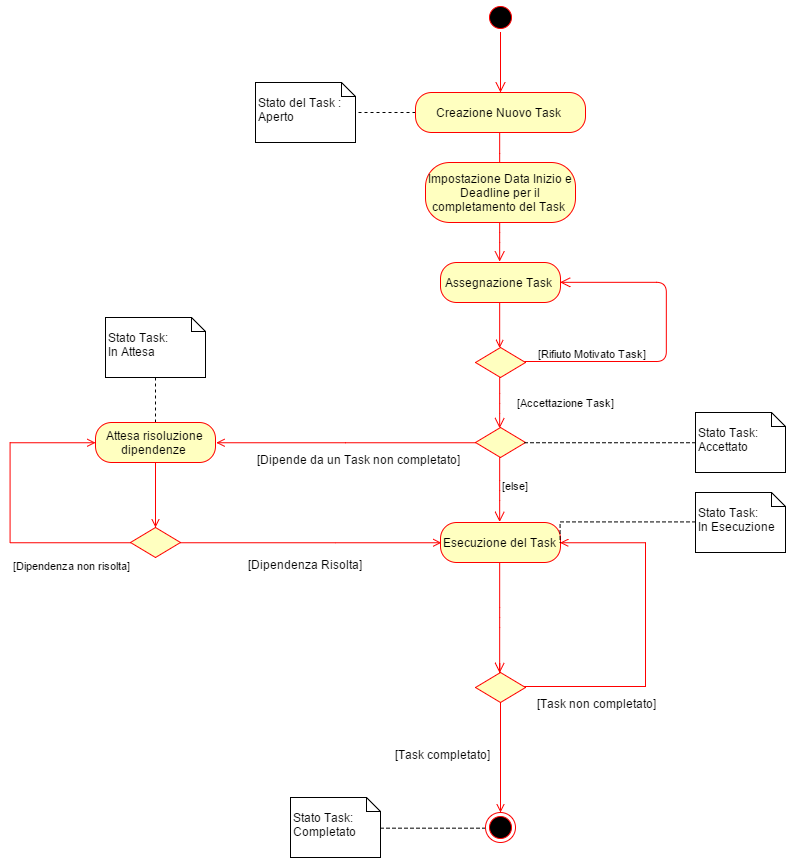
\includegraphics[scale=0.6]{TicketCicloVita.png}
		\caption{Diagramma del ciclo di vita dei ticket.}
	\end{figure}
\end{center}

\subsubsubsection{Ticket di Riunione}\label{ticketRiunione}
Un \mgls{ticket} di riunione è creato attraverso l'impostazione di un \mgls{evento} su \mGls{teamwork} e deve avere le seguenti caratteristiche:
\begin{itemize}

	\item \textbf{Titolo:} Riunione n. X, dove X indica il numero crescente di riunioni effettuate
	\item \textbf{Data:} la data del \mgls{ticket} dovrà essere impostata alla data prevista per la riunione
	\item \textbf{Ordine del Giorno:} elenco ordinato delle varie voci da esaminare sotto forma di commento al \mgls{ticket}
	\item Deve essere assegnato a tutti i membri del gruppo che sono invitati a partecipare alla riunione
\end{itemize}

\newpage

\appendix
\section{Lista di controllo}

Durante l’applicazione del \mgls{walkthrough} ai documenti, sono state riportate le tipologie di errori più frequenti. La lista di controllo risultante è la seguente:
\paragraph{Norme stilistiche}
\begin{itemize}

	\item elenco puntato: non inizia con la lettera maiuscola;
	\item elenco puntato: non termina con il punto e virgola oppure con il punto se è l’ultimo elemento;
	\item elenco numerato: non termina con il punto e virgola oppure con il punto se è l’ultimo elemento; 
	\item nome proprio di persona: non rispetta la norma Cognome Nome;
	\item nome ruolo di progetto: non viene utilizzata la macro predisposta;
	\item nome documento: non viene utilizzata la macro predisposta;
	\item "Proponente" e "Committente": non vengono scritte con la maiuscola iniziale. 
\end{itemize}

\paragraph{Italiano}
\begin{itemize}
	\item virgola tra soggetto e verbo: rende di difficile comprensione la frase;
	\item carattere "È": non viene scritto correttamente utilizzando il comando apposito;
	\item periodi: frasi troppo lunghe rendono i concetti di difficile comprensione; 
	\item doppie negazioni: evitare l’utilizzo di doppie negazioni perché complicano la comprensione della frase; 
	\item punto e virgola: evitare l’uso del punto e virgola quando è necessario usare il punto; 
	\item proponente e committente: non si deve confondere il loro significato. 

\end{itemize}


\paragraph{LaTeX}
\begin{itemize}
	\item se esiste una macro per definire il termine usare sempre la macro;
	\item lettere accentate nelle variabili: non viene utilizzato il comando apposito; 
	\item carattere di spaziatura: non deve essere utilizzato all'interno dei tag; 
	\item macro \LaTeX{}: non viene scritta usando l’apposito comando \latex{\textbackslash LaTeX}. 
\end{itemize}


\paragraph{UML}
\begin{itemize}
	\item il sistema non deve mai essere un attore; 
	\item controllo ortografico: deve essere effettuato in modo dettagliato a causa dell'impossibilità di automatizzare i controlli sui diagrammi; 
	\item direzione delle frecce non corrette; 
	\item consistenza della nomenclatura tra i diagrammi e le descrizioni testuali nei documenti. 
\end{itemize}

La seguente lista di controllo vuole riassumere invece gli  errori più frequenti rilevati durante il \mgls{walkthrough} del tracciamento requisiti effettuato mediante il software \mgls{tracy}:


\paragraph{Tracciamento requisiti}
La seguente lista vuole riassumere invece gli  errori più frequenti rilevati durante il \mgls{walkthrough} del tracciamento requisiti effettuato mediante il software \mgls{tracy}:
\begin{itemize}
	\item ad ogni caso d’uso deve corrispondere almeno un requisito;
	\item ad ogni requisito deve corrispondere almeno una fonte; 
	\item la fonte “Capitolato” non deve comparire nei requisiti interni; 
	\item deve esserci copertura totale del capitolato nei requisiti;
	\item devono essere impostate le corrette relazioni di parentela tra requisiti in \mgls{tracy}; 
	\item devono essere impostate le corrette relazioni di parentela tra casi d’uso in \mgls{tracy}; 
	\item in \mgls{tracy} deve essere indicato almeno un attore in ogni caso d’uso;
	\item controllare in \mgls{tracy} che le fonti dei requisiti siano le fonti corrette; 
	\item i codici dei casi d’uso nei diagrammi e in \mgls{tracy} devono corrispondere.
\end{itemize}


\newpage
\printglossary[title={Glossario}]

\end{document}
